
\chapter{The Braid Group and Anyons}\label{braids}

For our last group of study, we will focus our attention to a group of quite unique construction. We seek to make the idea of a braiding mathematically rigorous. We will be taking $n$ strands and tying them around each other to form new objects within our group. While this inherently concrete idea is our main goal to study, we require lots of rigorous mathematics to develop this concept sufficiently. Our ultimate goal is to begin characterization of a special kind of quasiparticle known as anyons. It turns out that when systems of anyons go through a processes that exchange their position, they exhibit behavior that resembles the structure of braids. We will utilize our study of representation theory to both study anyons through the perspective of braids and then study braids from the perspective of anyons. This chapter follows the structure of multiple sources, including Christian Kassel's \textit{Braid Groups}, Avinash Deshmukh's \textit{An Introduction to Anyons}, and Simon Trebst's \textit{A Short Introduction to Fibonacci Anyon Models}. \cite{Kassel,Deshmukh,Trebst}

\section{Construction of the Braid Group}

There are multiple ways to construct the braid group. While our instincts are to do so with the image of intertwined strings, we have to first a more algebraic definition to begin with.

\begin{definition}
	The braid group, $B_n$, is generated by $n-1$ generators (denoted $\sigma_1,\hdots,\sigma_{n-1}$) that have the following "braid relations":
$$\sigma_i\sigma_j = \sigma_j\sigma_i \hspace{3mm} \forall i,j \in \{1,\hdots,n-1\} \text{ where } |i-j|>1$$
$$\sigma_i\sigma_{i+1}\sigma_i=\sigma_{i+1}\sigma_i\sigma_{i+1} \hspace{3mm} \forall i \in \{1,\hdots,n-2\}$$
\end{definition}

These relations are somewhat daunting at first glance, but we can identify the braid group with a familiar group through the lens of a homomorphism to give us an easier interpretation for now. Consider the following map:

$$\phi:B_n\rightarrow S_n$$
$$\sigma_k \mapsto (k \hspace{2mm} k+1)$$

\noindent where $(k \hspace{2mm}k+1)$ is cycle notation for the transposition that swaps $k$ and $k+1$. This map can be shown to be a homomorphism, but most importantly, this map perserves the braid relations. That is to say, the transpositions of $S_n$ adhere to the braid relations. However we must be wary; these two groups are not the same. Namely, this is a result of the fact that every transposition is its own inverse in $S_n$ and none of the generators of $B_n$ are their own inverses. 

While this is a good way to get our bearings in the algebraic richness of the braid group, we can also construct this group in a more topological sense.

\begin{definition}
	A \textbf{geometric braid} on $n\in \N$ strands is a set $b\subset\R^2\times [0,1]$ formed by $n$ disjoint, intervals topologically equivalent to $[0,1]$ such that we can define a projection mapping from $\R^2\times [0,1]$ to $[0,1]$ that maps each strand homeomorphically to $[0,1]$ and the following conditions hold:
$$b\cap(\R^2\times\{0\}) = \{(1,0,0),(2,0,0),\hdots,(n,0,0)\}$$
$$b\cap(\R^2\times\{1\}) = \{(1,0,1),(2,0,1),\hdots,(n,0,1)\}$$
\end{definition}

\begin{figure}[H]
	\centering
	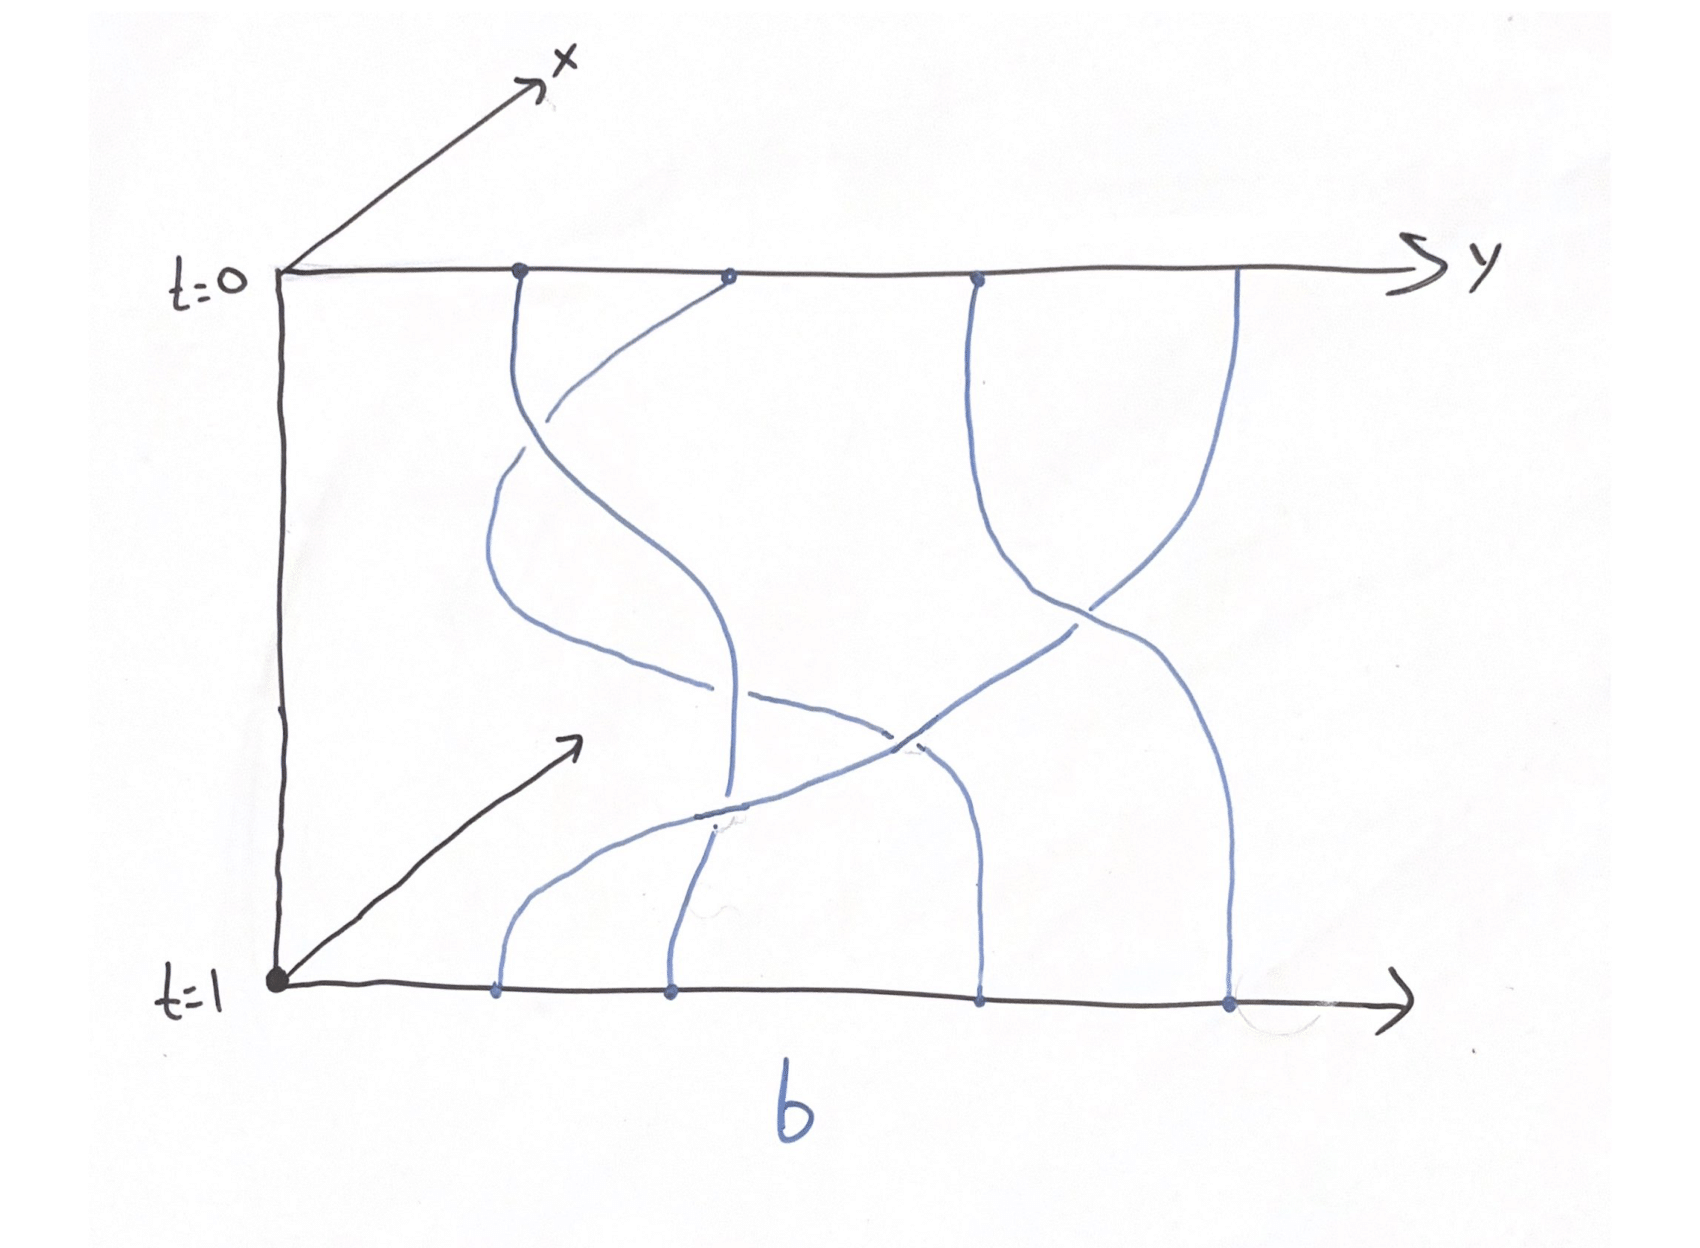
\includegraphics[width=0.7\textwidth]{geobraid.png}
	\caption{Generic geometric braid}
\end{figure}

Based on this construction of a braid, we can immediately notice a few properties. First, every stand will intersect a level curve of this set at exactly one point (otherwise the stands are not homeomorphic to $[0,1]$). Further, every strand can be traveled as a path, having a unique start and end point. If each strand begins at the point $(n,0,0)$ and ends at $(n',0,1)$, then we can construct a permutation in $S_n$ that captures the behavior of this transition (from $n$ to $n'$). We call such a permutation the underlying permutation of $b$.

\begin{definition}
	Two braids, $b_1$ and $b_2$, are said to be \textbf{isotopic} to each other if one can be continuously deformed into the other. This is an equivalence relation.
\end{definition}

We can define the product between two braids heuristically and formally. Crudely, the product of two braids is defined to be the stacking of one braid on top of the other, lining up the start and end points. More formally, if $b_1$ and $b_2$ are two geometric braids, we define 

\begin{equation}
\begin{aligned}
	b_1b_2 \coloneq \{(x,y,t)\mid (x,y,2t)\in b_1 \text{ when }0\leq t\leq \frac{1}{2} \text{ and }   (x,y,2t - 1)\in b_2 \text{ when }\frac{1}{2}\leq t\leq 1\}
\end{aligned}
\end{equation}

\begin{figure}[H]
	\centering
	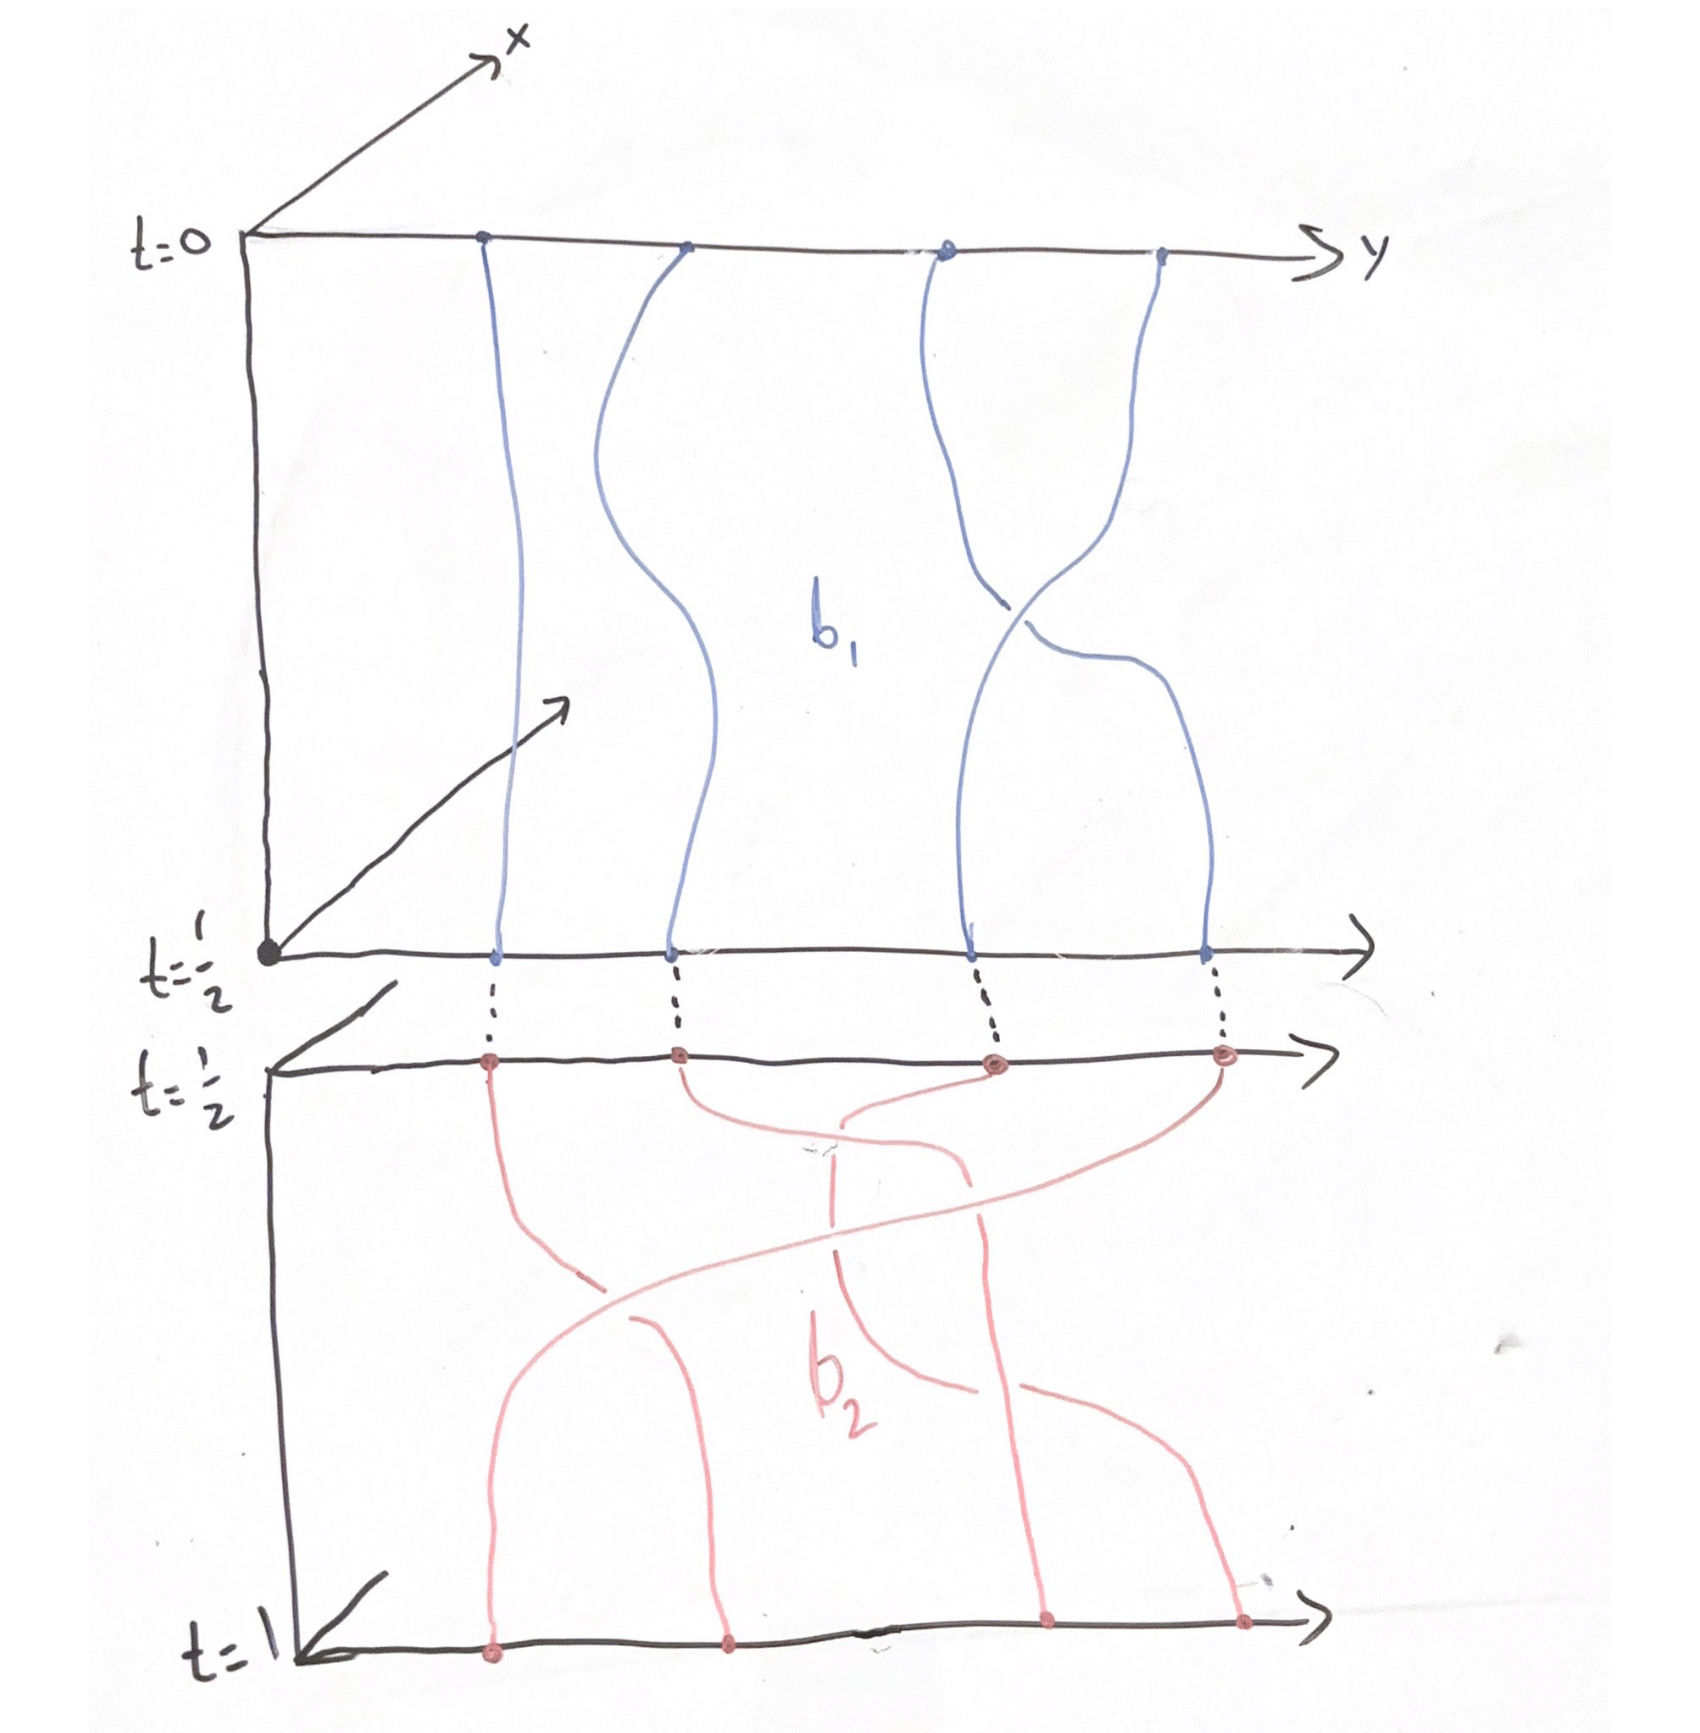
\includegraphics[width=0.7\textwidth]{geobraidprod.png}
	\caption{The product of two geometric braids.}
\end{figure}

This operation is clearly associative, and there is an identity element corresponding to the geometric braid that does not wrap any strands around one another. Hence, the collection of all geometric braids forms a group. To avoid any unecessary craziness, we will work on the group of equivalence classes of geometric braids. We will work towards establishing the connection the canonical braid group $B_n$ and the group of geometric braids.

In order to visualize more easily, we will formally introduce the concept of a braid diagram.

\begin{definition}
	A \textbf{braid diagram} on $n$ strands is set, $\mathcal{D}\subset \R\times [0,1]$ made up as a union of $n$ intervals topologically equivalent to $[0,1]$ (called strands) such that the following conditions are met:
\begin{itemize}
	\item There exists a projection map from $\R\times [0,1]$ to $[0,1]$ that maps each strand homeomorphically to $[0,1]$.
	\item Every element of $\{1,2,\hdots,n\}\times\{0,1\}$ is a starting or endpoint of a unique strand.
	\item Every element in $\mathcal{D}$ belongs to either one or two strands. When an elment belongs to two, one strand must be designated as overgoing and the other undergoing (referred to as a crossing of $\mathcal{D}$
\end{itemize}
\end{definition}

We can make an intuitive identification of geometric braids with braid diagrams by thinking of the latter as a projection of the former onto the $xt$-plane ($t$ representing the interval $[0,1]$). Identifying a geometric braid with a braid diagram takes the diagram and at every crossing, splits the strands in such a way that the undergoing strand gets placed ``behind" the overgoing strand, which there is plenty of room to do in $\R$.

Much like the braids the that braid diagrams represent, two braid diagrams are said to be isotopic if one can be continuously deformed into the other. Further, we can define a product on braid diagrams as well in an identical process that we did to define it on the braids. The product of two braid diagrams visually resembles stacking two diagrams on top of each other. In this way, we can  identify the group of geometric braids with a carefully group of braid diagrams (of course defined on equivalency classes in both settings). 

However, these groups are not necessarily isomorphic. When projecting down in onto a two-dimensional surface, we lose information about the geometric braid. There is potential to confuse two braid diagrams as representing different geometric braids when in reality they represent an isotopic geometric braid.

\begin{figure}[H]
	\centering
	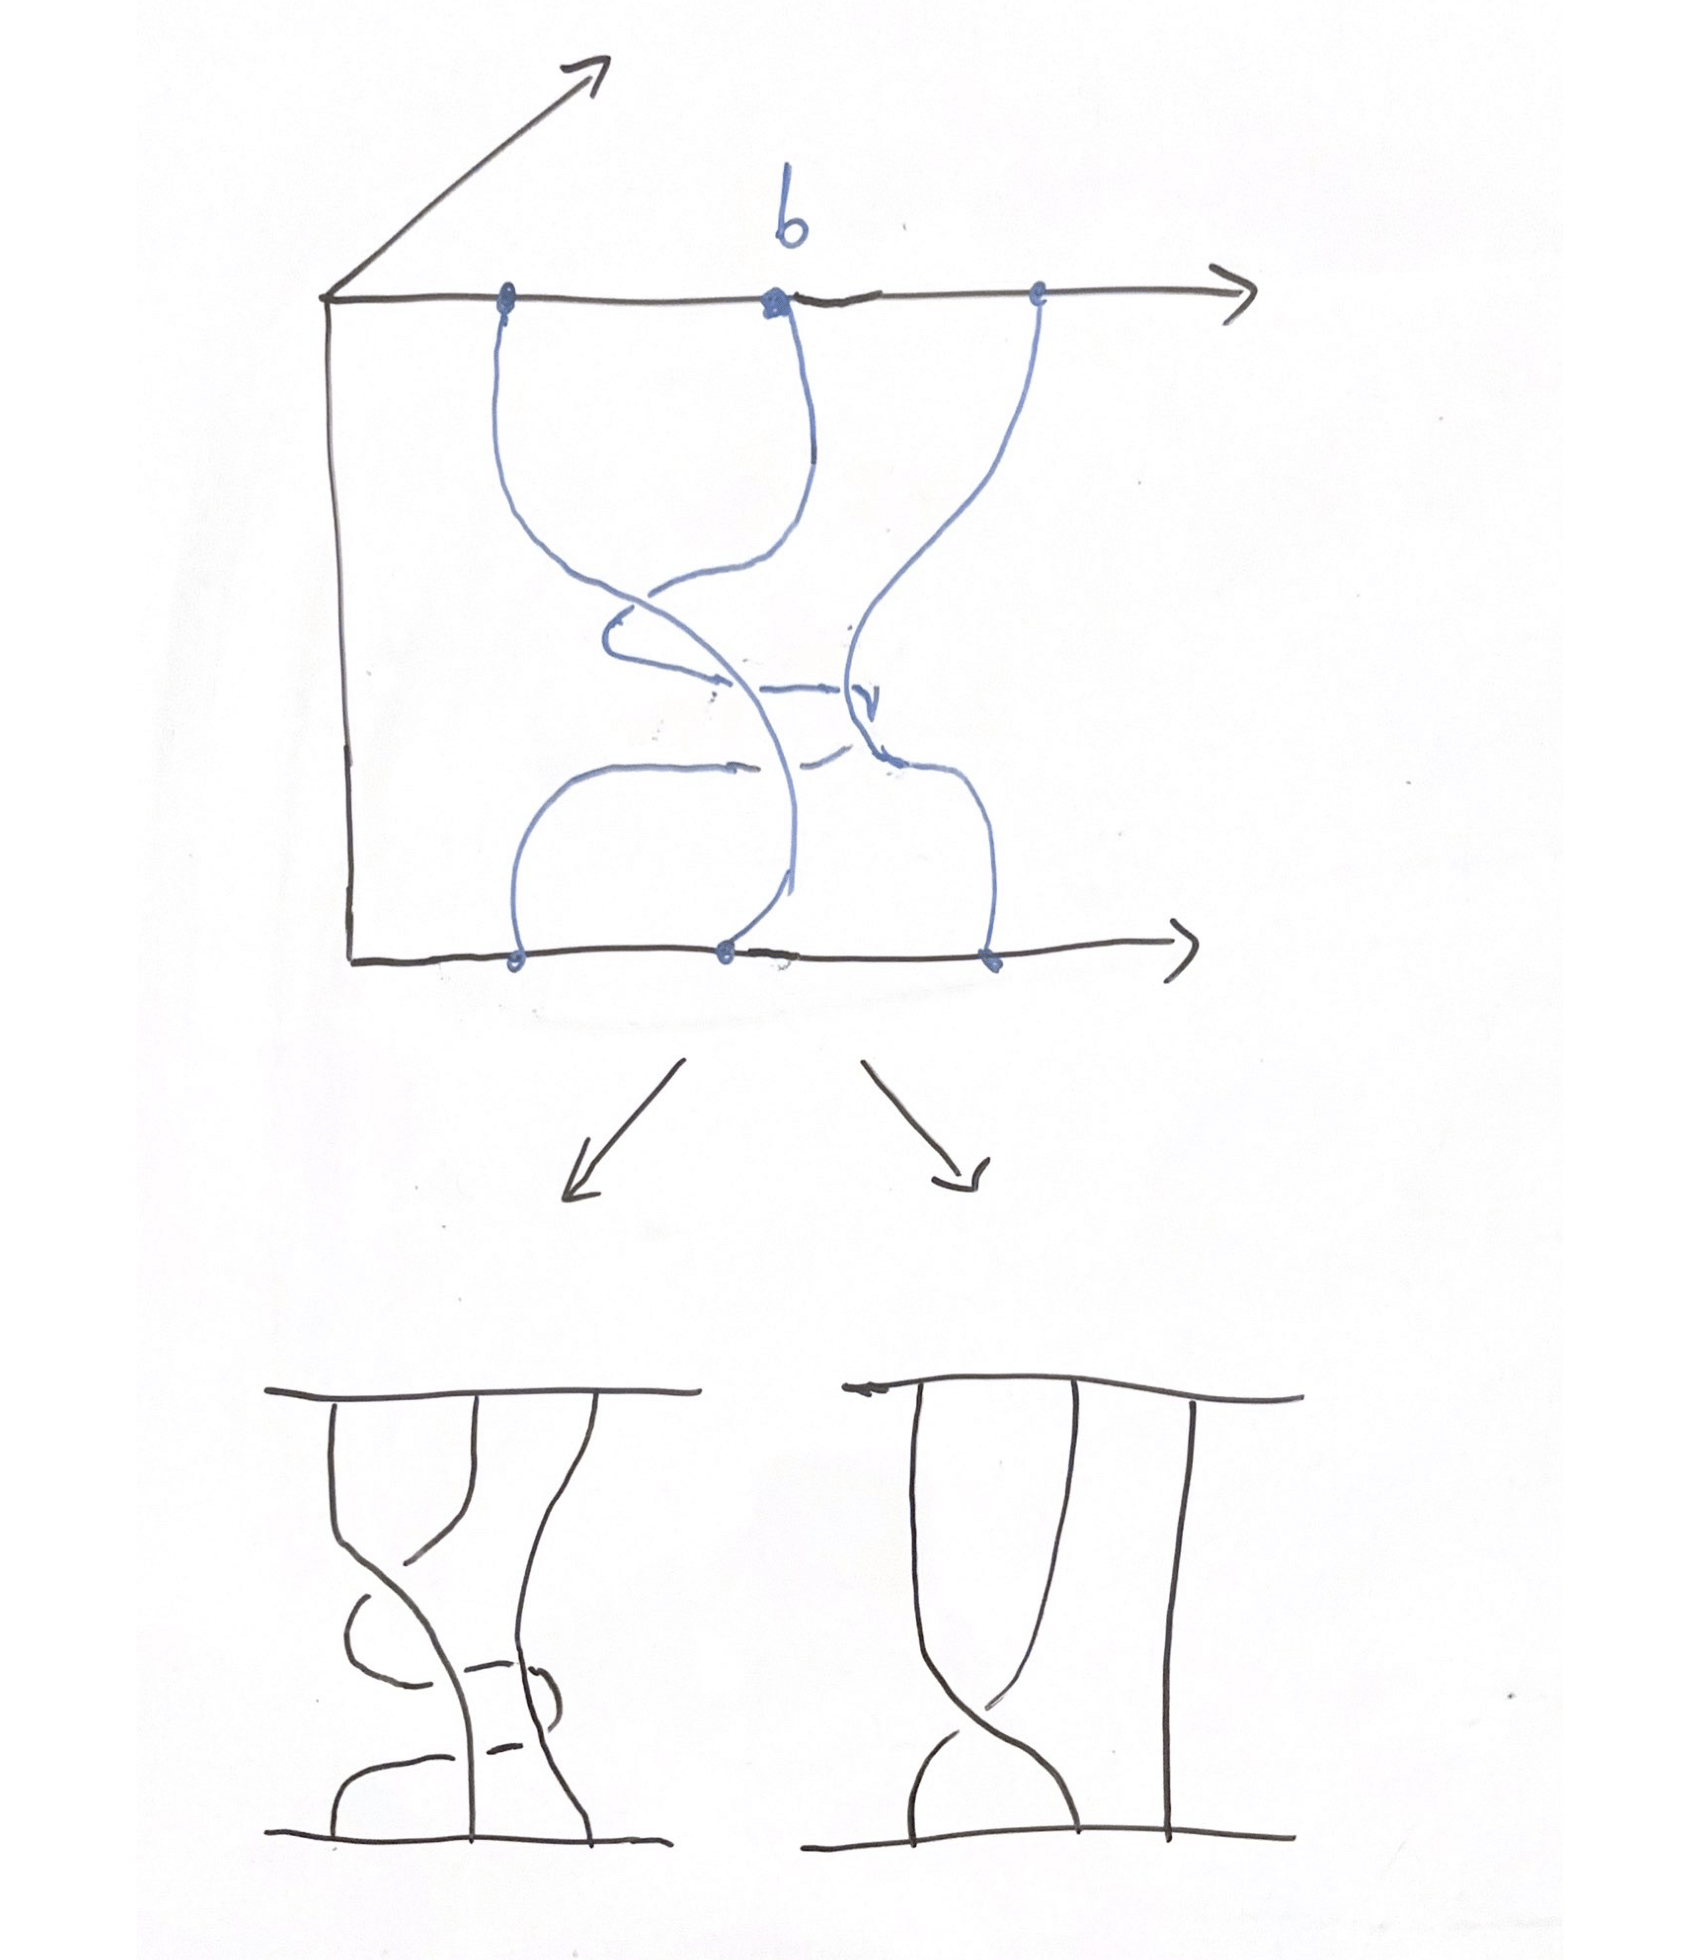
\includegraphics[width=0.7\textwidth]{requiv.png}
	\caption{Two braid diagrams that correspond to the same geometric braid.}
\end{figure}

We appeal to the Reidemeister moves developed in Knot Theory to aid us in our ability to detect when braid diagrams represent the same geometric braid. There are two specific types of moves we will reference.

Our first kind Reidemeister move to be consider will be given the label $\Omega$. Applying the move $\Omega$ to two adjacent strands of a braid does the following: First, it chooses one strand to be the overgoing strand and the other to be the undergoing strand. Then it takes the overgoing strand and creates two crossings by moving part of the strand over and across the other strand. There are two crossings because the strands are not switching positions, meaning the path the strand makes must return back the way it came. Note that we have to make a choice about which strand is under-versus-overgoing, and so we will take the convention that $\Omega_1$ is the move that favors the left strand as overgoing and $\Omega_2$ is the move that favors the right as overgoing. The inverses of both these moves are also Reidemeister moves.

\begin{figure}[H]
	\centering
	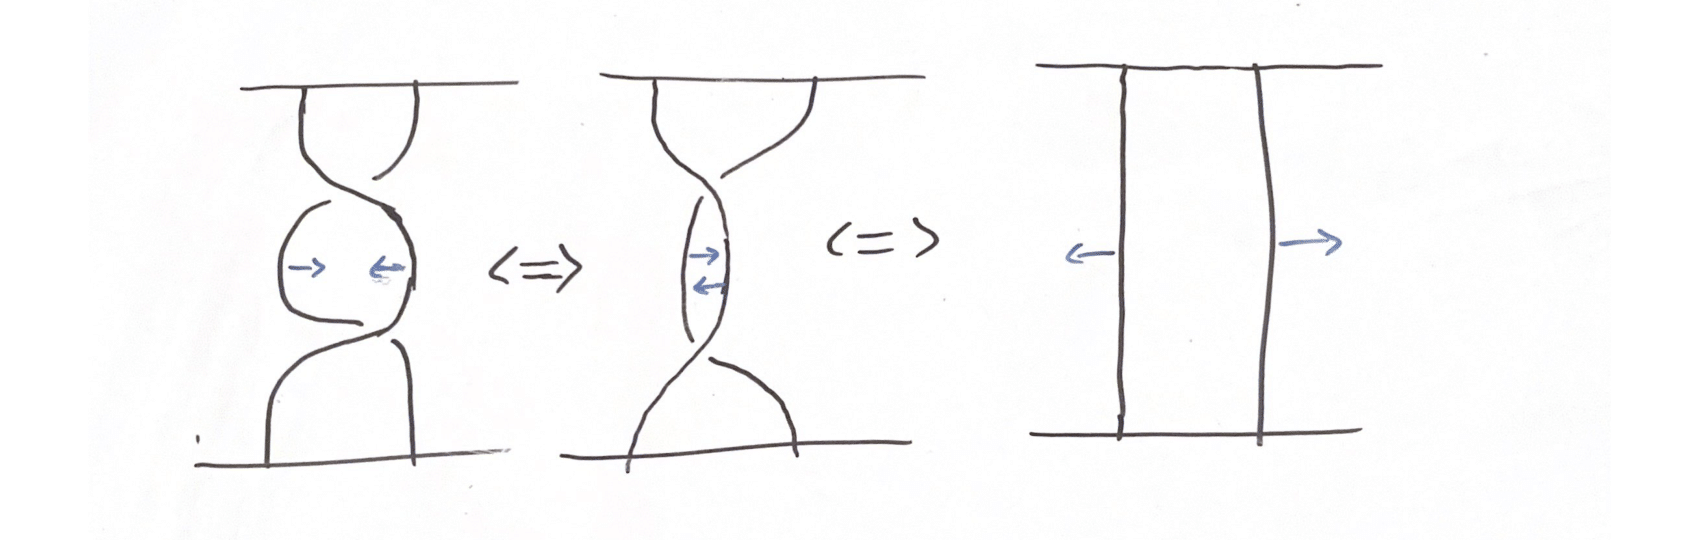
\includegraphics[width=0.7\textwidth]{reidmove2.png}
	\caption{$\Omega_1^{-1}$}
\end{figure}

Our second kind of Reidemeister move will be given the label of $\Theta$. In order to execute this move, we require there be three adjacent strands. Further we need one strand to cross both other strands in the same manner (simultaneously under-or-overgoing) and that the remaining two strands cross in an unspecified manner. The move $\Theta$ will take the one strand that under/overgoes both and moves it under/over the crossing of the other two strands to the other side. 

\begin{figure}[H]
	\centering
	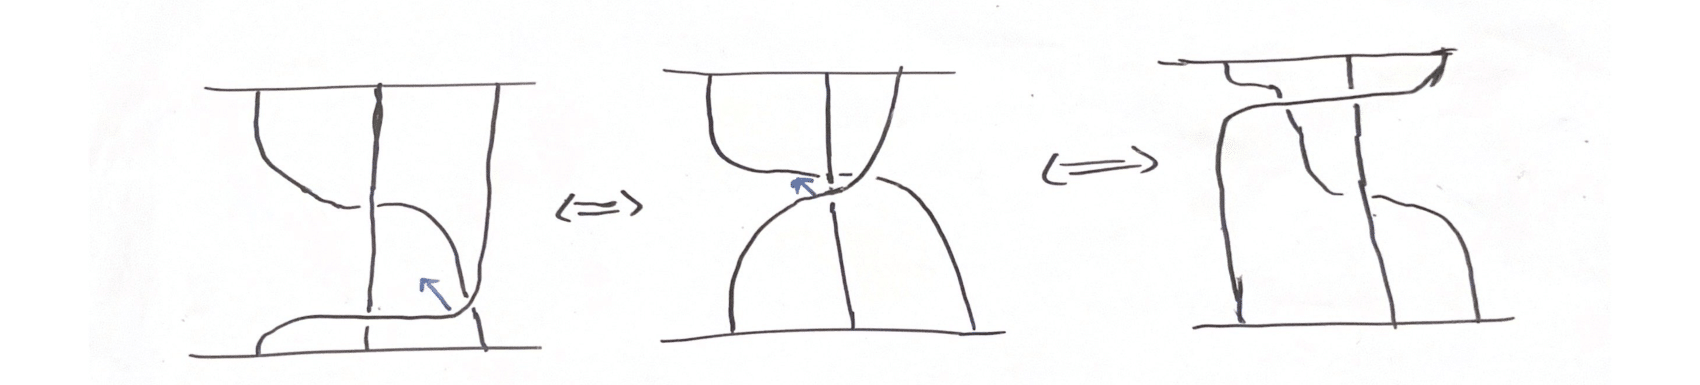
\includegraphics[width=0.7\textwidth]{reidmove3.png}
	\caption{$\Theta$}
\end{figure}

\begin{definition}
	Two braid diagrams are said to be \textbf{R-equivalent} if one can be transformed into the other by means of a finite sequence of isotopies and Reidemeister moves.
\end{definition}

R-equivalence is naturally an equivalence relation, and if we consider the quotient space of the group of braid diagrams, we get a group isomorphic to the group of geometric braids.

Now, all that is left to do is connect our geometric braids back to the algebraic definition. We can start by considering the braid diagrams of our geometric braids. If we are considering braids on $n$ strands, then we define $\sigma_i^+$ to be the braid diagram where the only crossing is the $i^{th}$ strand crossing under the $i+1^{th}$ strand and $\sigma_i^-$ to be the braid diagram where the only crossing is the $i^{th}$ strand crossing over the $i+1^{th}$ strand. We define this for ever $i\in\{1,2,\hdots,n-1\}$. Then the following holds:

\begin{theorem}
	Let $\mathcal{B}_n$ be the group of geometric braids on $n$ strands. Then for any $\beta\in\mathcal{B}_n$, $\beta$ has a natural decomposition:
$$\beta = \sigma^{\epsilon_1}_{i_1}\hdots\sigma^{\epsilon_k}_{i_k}$$ 
where $i_1,i_2,\hdots,i_k\in\{1,2,\hdots,n-1\}$ and $\epsilon_i = \pm$
\end{theorem}

\noindent \begin{proof}\cite{Kassel}  Let $D(\beta)$ be the braid diagram of $\beta$. Then, we can create a partition of the interval $[0,1]$ in such a way that for every subinterval indicated by the partition, only one crossing occurs. Each subinterval thus defines a braid diagram where only one crossing occurs, which is defined to be $\sigma_i^\epsilon$ for some $i\in\{1,2,\hdots,n-1\}$ and some $\epsilon = \pm$. Since products of braid diagrams are crudely defined as a stacking of braids on top of one another, we can recover the entire diagram of $D(\beta)$ by considering it as a product of the diagrams defined by the subintervals. This brings us to our desired result of 

\begin{equation}
\begin{aligned}
\beta = \sigma^{\epsilon_1}_{i_1}\hdots\sigma^{\epsilon_k}_{i_k}  
\end{aligned}
\end{equation}
\end{proof}

\begin{corrolary}
	Any $\beta\in\mathcal{B}_n$ has a well defined inverse in $\mathcal{B}_n$.
\end{corrolary}

\noindent\begin{proof}\cite{Kassel}  If $\beta = \sigma^{\epsilon_1}_{i_1}\hdots\sigma^{\epsilon_k}_{i_k}$, then $\beta = \sigma^{-\epsilon_k}_{i_k}\hdots\sigma^{-\epsilon_1}_{i_1}$ \end{proof} 

\begin{theorem}
	The following map is an isomorphism of groups:
$$\phi:\mathcal{B}_n\rightarrow B_n$$
$$\sigma_i^+ \mapsto \sigma_i$$
\end{theorem}

\noindent\begin{proof}\cite{Kassel}  Since $\phi$ is defined on generators, it must naturally inheret homomorphism properties. 

(Surjective) Since $\phi$ maps to every generator of $B_n$, the map is automatically surjective.

(Injective) Let $\psi:B_n\rightarrow\mathcal{B}_n$, $\sigma_i\mapsto\sigma_i^+$. Injectivity is dependent on whether or not this map is the identity map. Then, for any element, $\beta\in\mathcal{B}_n$, $\psi(\phi(\beta)) = \sigma^{\epsilon_1}_{i_1}\hdots\sigma^{\epsilon_k}_{i_k}$. If this construction perserves R-equivalence, then we are done. Reidemeister rules are straigforward to check. Our $\Omega$ moves at terms of $\sigma_i^+\sigma_i^-$ which is the identity. Our $\Theta$ moves exchange $\sigma_i^+\sigma_{i+1}^+\sigma_i^+$ with $\sigma_{i+1}^+\sigma_i^+\sigma_{i+1}^+$ which are equivalent given our braid relations. Finally, isotopies only exchange the order in which the terms in the decomposition would occur as long as the strands are not adjacent (which the braid relations assert are equivalent). Therefore, this image under the composition is the same $\beta$ we started with! \end{proof} 

\section{The Burau Representation}


In the past, we have considered representations where the matrices have been defined to have entries in a field. For our discussion of this representation however, we will relax our definition to allow for entries in generic rings to be acceptable. To this end, we consider matrices in $M_n(\Z[t,t^{-1}])$ where $\Z[t,t^{-1}]$ is the ring of Laurant polynomials with integer coefficients. For a fixed $n>2\in\N$, we define the following block diagonal matrices for all $i\in \{1,\hdots,n-1\}$

\begin{equation}
\begin{aligned}
U_i = \begin{bmatrix}
			I_{i-1}& 0 & 0 & 0 \\
			0 & 1-t & t & 0\\
			0 & 1 & 0 & 0\\
			0 & 0 & 0 & I_{n-i-1}
		\end{bmatrix}
\end{aligned}
\end{equation}

Based on this construction, there are a few things worth noting immediately. First, $U_1$ has no identity block in the top left corner and $U_{n-1}$ has no block in the bottom right corner. The next noteworthy observation to make is that this complicated construction is actually somewhat simpler than it appears at first glance. If we make the substitution $t=1$ into this matrix, we would have a permutation matrix. More specifically, we have a matrix corresponding to a transposition of adjacent indices, which happens to be what the image of the generators of the braid group are under the map defined near Definition (6.1). Lastly, the most relevant feature of these matrices is the middle block. Since the entire matrix acts as an identity matrix aside from this $2\times 2$ block, the key to studying these matrices in more detail lies here.

Setting $U= \begin{bmatrix} 1-t & t\\1 & 0 \end{bmatrix}$, we use the Cayley-Hamilton theorem to conclude that

\begin{equation}
\begin{aligned}
	U^2 - (1-t)U - tI_2 = 0
\end{aligned}
\end{equation}

The identity matrix happen to also satisfy this equation, and therefore we can generally claim that 

\begin{equation}
\begin{aligned}
	U_i^2 - (1-t)U_i - tI_n = 0
\end{aligned}
\end{equation}

which can be rewritten as 

\begin{equation}
\begin{aligned}
	U_i(\frac{1}{t}U_i - \frac{1}{t}(1-t)I_n) =I_n 
\end{aligned}
\end{equation}

Showing that $U_i$ is invertible with an explicit formula:

\begin{equation}
\begin{aligned}
	U_i^{-1}=\begin{bmatrix}
			I_{i-1}& 0 & 0 & 0 \\
			0 & 0 & 1 & 0\\
			0 & \frac{1}{t} & 1-\frac{1}{t} & 0\\
			0 & 0 & 0 & I_{n-i-1}
		\end{bmatrix}
\end{aligned}
\end{equation}

which is established just the way we expect it to be.

It is also worth noting that these matrices satisfy the braid relations. That is, $U_iU_j=U_jU_i$ commute when $|i-j|>1$ (which is clear when we notice that the nontrivial blocks do not coincide when this condition is met) and $U_iU_{i+1}U_i=U_{i+1}U_iU_{i+1}$ $\forall i\in\{1,\hdots,n-2\}$ (which can be confirmed by matrix algebra).

\begin{definition}
	The \textbf{Burau Representation} of $B_n$ is the map 
$$\phi_n:B_n\rightarrow M_n(\Z[t,t^{-1}])$$
$$\sigma_i \mapsto U_i$$
\end{definition}

It turns out that this representation can lead us to the creation of a unitary representation. We will proceed to aruge this as follows. Consider the following $n\times n$ matrix

\begin{equation}
\begin{aligned}
	\Omega_n = \begin{bmatrix}
						1 & 0 & 0 &\hdots & 0 \\
						1-t & 1 & 0 & \hdots & 0 \\
						1-t & 1-t & 1 & \hdots & 0 \\
						\vdots&\ddots&\ddots&\hdots&\vdots\\
						1-t & 1-t & 1-t & \hdots & 1
					\end{bmatrix}
\end{aligned}
\end{equation}\\

\begin{theorem}
	For any $M\in \phi_n(B_n)$, 
$$\overline{M}\Omega_nM^\intercal = \Omega_n$$
where $\overline{M}=[\overline{M_{ij}}]$ where the conjugate bar maps $t$ to $\frac{1}{t}$.
\end{theorem}

\noindent\begin{proof}\cite{Kassel}  It suffices to prove this statement for the image under generators of $B_n$. If we let $K_{m,n}$ be the matrix of dimension $m\times n$ filled with the entry $1-t$, we can consider the decomposing the matrix $\Omega_n$ into a block structure consistent with the blocks of the image of one generator. Let $i\in\{1,\hdots,n-1\}$. Then consider 

\begin{equation}
	\begin{aligned}
		\Omega_n = \begin{bmatrix}
							\Omega_{i-1} & 0 & 0\\
							K_{2,i-1} & \Omega_2 & 0 \\
							K_{n-i-1,i-1}& K_{n-i-1,2}&\Omega_{n-i-1}
						\end{bmatrix}
	\end{aligned}
\end{equation}
\begin{equation}
	\begin{aligned}
		M = U_i = \begin{bmatrix}
							I_{i-1} & 0 & 0\\
							0 & U & 0 \\
							0& 0&I_{n-i-1}
						\end{bmatrix}
	\end{aligned}
\end{equation}

Then

\begin{equation}
	\begin{aligned}
		\overline{M}\Omega_nM^\intercal = \begin{bmatrix}
														\Omega_{i-1} & 0 & 0\\
														\overline{U}K_{2,i-1} & \overline{U}\Omega_2U^\intercal & 0 \\
														K_{n-i-1,i-1}& K_{n-i-1,2}U^\intercal&\Omega_{n-i-1}
													\end{bmatrix}
	\end{aligned}
\end{equation}

It can be shown that $\overline{U}K_{2,i-1} = K_{2,i-1}$ and $K_{n-i-1,2}U^\intercal=K_{n-i-1,2}$. All that's left to calculate is 


\begin{equation}
	\begin{aligned}
		\overline{U}\Omega_2U^\intercal &= \begin{bmatrix}
													1-\frac{1}{t} & \frac{1}{t}\\
													1 & 0 
													\end{bmatrix}
													\begin{bmatrix}
													1 & 0\\
													1-t & 1 
													\end{bmatrix}
													\begin{bmatrix}
													1-t & 1\\
													t & 0 
													\end{bmatrix}\\
												&= \begin{bmatrix}
													1-\frac{1}{t} & \frac{1}{t}\\
													1 & 0 
													\end{bmatrix}
													\begin{bmatrix}
													1-t & 1\\
													(1-t)^2 + t & 1-t 
													\end{bmatrix}\\
												&= \begin{bmatrix}
													1 & 0\\
													1-t & 1 
													\end{bmatrix} \\
												&= \Omega_2
	\end{aligned}
\end{equation}

Therefore, our substitution of these matrices into their respective blocks gives us our desired results. \end{proof} 

Taking the "conjugate"-transpose of both sides of this theorem's result gives us an identical formulation:

\begin{equation}
	\begin{aligned}
		\overline{M} \overline{\Omega_n}^\intercal M^\intercal = \overline{\Omega_n}^\intercal
	\end{aligned}
\end{equation}

We can add these two equations together in order to obtain

\begin{equation}
	\begin{aligned}
		\overline{M}(\Omega_n + \overline{\Omega_n}^\intercal )M^\intercal = \Omega_n + \overline{\Omega_n}^\intercal 
	\end{aligned}
\end{equation}

If we define a new matrix in terms of our $\Omega_n$ matrices:
\begin{equation}
	\begin{aligned}
		\Theta_n &= \Omega_n + \overline{\Omega_n}^\intercal \\
					&=  \begin{bmatrix}
						2 & 1-\frac{1}{t} & 1-\frac{1}{t} &\hdots & 1-\frac{1}{t} \\
						1-t & 2 & 1-\frac{1}{t} & \hdots & 1-\frac{1}{t} \\
						1-t & 1-t & 2 & \hdots & 1-\frac{1}{t} \\
						\vdots&\ddots&\ddots&\hdots&\vdots\\
						1-t & 1-t & 1-t & \hdots & 2
					\end{bmatrix}
	\end{aligned}
\end{equation}

It is clear that $\overline{\Theta_n}^\intercal = \Theta_n$, illustrating that this matrix is "Hermitian." We now have all that we require to transform the Burau representation into a classical unitary representation.

Let $\zeta$ be a complex number with $|\zeta|=1$. $p_\zeta:\Z([t,t^{-1}]) \rightarrow \C$ be the ring homomorphism defined to send $t\mapsto\zeta$. If we apply this map entry-wise on our matrices, the act of conjugation as we defined on the matrices has the same effect as complex conjugation. To this end, we can define the representation:

$$P_\zeta = p_\zeta\circ\phi_n: B_n\rightarrow GL_n(\C)$$

Selecting $\zeta=1$ gives us the $p_\zeta(\Theta_n) = 2I_n$, and therefore the identity derived in (6.14) becomes

\begin{equation}
	\begin{aligned}
		\overline{P_\zeta(\beta)}P_\zeta(\beta)^\intercal = I_n &\\
		\Leftrightarrow P_\zeta(\beta)\overline{P_\zeta(\beta)}^\intercal  = I_n
	\end{aligned}
\end{equation}

Therefore, we have uncovered a unitary representation of $B_n$

\section{Anyons and their Relation to the Braid Group}

We begin our discussion of anyons by first analyzing the general set-up. We will be viewing these problems through the lens of quantum mechanics. As a general practice, the study of quantum mechanics takes the form of studying functions that represent a system of subatomic particles (in our case anyons). We refer to such functions as "wave functions." Wave functions are a catch all for describing every phenomenon occuring in the system at a given moment in time. As such, we think to each wave function as representing the state of a system. Even though these functions are dependent on time, in our analysis, we will regard time as a fixed quantity (we analyze our states in a specific instance in time). The dependence of the system therefore relies on other characteristics, like the number of particles, each particle's respective properties, etc. As such, any wave function will be defined entirely based on the instantaneous physical properties of the objects we study. Despite these differences, the fundamental idea of what wave functions represent remains the same. In the study of quantum mechanics, we embrace an element of stochasticity in the way our particles are defined: we never actively know where a particle is unless we measure it empirically. To this end, any wave function, $\psi$, is constructed to measure the ambiguity in the following way:

\begin{equation}
	\begin{aligned}
		\int_\Omega |\psi|^2 d\mu = 1
	\end{aligned}
\end{equation}

The interpretation for this property is that $|\psi|^2$ acts as a probability density function for our quantum system. For a specific example, if we use the positions of particles as the inputs of a wave function, we can compute the probability that our particles fall a specific region using the above condition. In general, this class of functions is somewhat broad; any particles in a quantum system (regardless of what kind of particle they are) have $100\%$ chance of being in the space we are considering. So, in an effort to simplify our exploration, let us rigorously define the space of wave functions we will be working in. Suppose that we have a two particle quantum system in which both of our particles are indistinguishable. That is to say we have no way to tell one apart from the other, not even based on their position. All of their intrinsic properties must be considered as equivalent. We will then consider each particle's position as an independent variable. Our interpretation of (6.17) will therefore be a probability that both our particles fall within a specified region. These wave functions will intuitively come from the Hilbert space $L^2(\C^2)$ and be normalized with respect to the $2-norm$. It is clear that this a vector space, and that any linear combination of functions in this space can be normalized to form new wave functions. This process is referred to as quantum superposition and will be revisited as we develop our work. Briefly, superpositions of wave functions inherently have coefficients (after normalization) that corresponds the probability that the given state will "collapse" into its corresponding summand. That is to say, every quantum superposition is a weighted sum of distinct states with coefficients equal to the probability that the superposition will when measured by observed as a its corresponding state.

An immediate observation we can make about this set up concerns the equivalence of states. It is clear that if we have the wave function, $\psi$, then for any complex number of the form $e^{i\theta}$,

\begin{equation}
	\begin{aligned}
		|e^{i\theta}\psi(r_1,r_2)|^2 = |\psi(r_1,r_2)|^2 
	\end{aligned}
\end{equation}

As a result, any integration over either function will yield the same value. These wave functions therefore must represent the exact same state. If we wish to reference (normalized) functions in $L^2(\C^2)$ as distinct wave functions, we can construct the a quotient space to this end. If we define an equivalence relation, $\sim$, by asserting two functions are related if one is a non-zero scalar multiple of the other, we can construct our space of interest:

\begin{equation}
	\begin{aligned}
		H \coloneq L^2(\C^2)/\sim
	\end{aligned}
\end{equation}

this type of space is sometimes referred to as a projective Hilbert space, where elements (referred to as rays) are one-dimensional subspaces of the original Hilbert space. We can choose a unit representative to be the wave function represented by the wave function of interest. We refer to the value $e^{i\theta}$ as the global phase of the wave function.

With all this set up in mind we can easily construct our vector space(s) of interest for the rest of this section. In general, we will constuct an $n$-dimensional vector space, $V$, to be the span of distinct $\psi_1,\hdots,\psi_n\in H$. We will always take the unit representative in $H$ for each choice of basis vector in $V$. This construction is necessary in order to focus on a finite-dimensional vector space, since $H$ is infinite dimensional. While our space will always be finite dimensional, since our choice of basis vectors is arbitrary, we can still make wide reaching conclusions. 

For our initial exploration of these spaces, let $V = span\{\psi\}$ as perscribed above. We characterize this state ($\psi$) by our recollection that the system we are studying is a two particle system where particles are indistinguishable ($\psi:\C^2\rightarrow\C^2$). While the classification of particles being indistinguishable appears to make our problem more difficult, it will actually lead to an interesting simplification. If we consider the first input ($r_1$) to track the position of particle one and the second input ($r_2$) to track the position of particle two, then we make the following crude interpretation:

\begin{small}
\begin{equation}
	\begin{aligned}
		\int_B \int_A |\psi(r_1,r_2)|^2 d\mu(A)d\mu(B) \sim \text{ The Probability that particle one is in A and particle two is in B}
	\end{aligned}
\end{equation}
\end{small}

where $A,B\subset\C$. Given that the nature of indistinguishable particles, we cannot be able to tell whether or not two particles switch places at any given state. If we did have a way to deduce this, our particles would be abe to be distinguished from one another. Therefore, it should not make a difference if we assert that particle one is in the set $A$ and particle two in set $B$ versus particle one being in set $B$ and particle two being in set $A$. Explicitly,

\begin{equation}
	\begin{aligned}
		\underset{\text{Particle one is in A and Particle two is in B}}{\int_B \int_A |\psi(r_1,r_2)|^2 d\mu(A)d\mu(B)} = \underset{\text{Particle one is in B and Particle two is in A}}{\int_B \int_A |\psi(r_2,r_1)|^2 d\mu(A)d\mu(B)}
	\end{aligned}
\end{equation}

Since $A$ and $B$ are arbitrary, we conclude that 

\begin{equation}
	\begin{aligned}
		|\psi(r_1,r_2)|^2 = |\psi(r_2,r_1)|^2 \hspace{3mm}a.e.
	\end{aligned}
\end{equation}

or rather,

\begin{equation}
	\begin{aligned}
		\psi(r_1,r_2) = e^{i\theta} \psi(r_2,r_1) \hspace{3mm}\text{for some }\theta\in[0,2\pi) \hspace{1mm} a.e.
	\end{aligned}
\end{equation}

In this way, we can classify our particles based on the choice of $\theta$, where the factor is sometimes referred to the relative phase of a wave function (when the phase is observed in comparison to another wave function). If we make the assumtion that the process of swapping these particles brings the state back to of its original state, then swapping the two particles a second time will result in the following 

\begin{equation}
	\begin{aligned}
		\psi(r_1,r_2) = e^{2i\theta} \psi(r_1,r_2) \hspace{3mm}\text{for some }\theta\in[0,2\pi) \hspace{1mm} a.e.
	\end{aligned}
\end{equation}

meaning that $\theta = 0,\pi$. Thus we have a natural split characterizing two different classes of particles. In the $\theta=0$ case, this wave function characterizes the state of two bosons. The category of bosons consists of many kinds of subatomic particles or composites of them. Many bosons are characterized as "force-carrying" and are responsible for particles experiencing forces that act on each other. The other case, $\theta=\pi$, charaterizes the state of two fermions. Fermions are generally thought of as classifying the kind of particles that make up basic components of matter. Examples include the classical protons, neutrons, electrons, and more. An inherent property of fermions, which is not necessarily true for bosons is their intrinsic need to not take up the same space (which is evidenced by the above wave function). This is actually responsible for many of the chemical properties that force atomic structure into place.

In order to assert these two particles have the following behavior, we had to know that transposing the particles twice would lead us to have the same state. However, there are some cases in which this assumption cannot be made, specifically in two-dimensions. In this way, there is a sort of ``memory" that these particles have, in that their relative phase with respect to one another is dependent on all previous particle exchanges. As a result, arbitrary permutations of our inputs need not ever return the value of the wave function back to its initial phase. We call such particles anyons.

For a moment, let us extend our construction of the space of wave equations to include $n$ anyon particles. In this case, wave functions are normalized elements of $L^2(\C_n)$. From a physical stand point, it is clear that exchanging two particles and then exchanging two different particles (no overlap in particles selected for exchange from either swap) can happen in any order without changing to acheive an identical state. In other words, swapping particles is a commutative action unless the swaps utilize some of the same particles. Further, the braid relation $\sigma_i\sigma_{i+1}\sigma_i =\sigma_{i+1}\sigma_i\sigma_{i+1}$ can be viewed in the context of particle exchange. Physical properties of the system allow us to conclude that this relationship must be satisfied by anyons. Therefore, we can homomorphically identify the generators of the braid group on $n$ particles with exchanges of adjacent, indistinguishable particles in a quantum system.

Now that we have identified the connection between the braid group and anyon particle exchange, we can immediately write down our first irreducible representation. If the exchange of anyons scales the wave function by a phase of $e^{i\theta}$, we say that the anyons ``obey $\theta$ statistics". Then, we can construct an irreducible representation for any anyons obeying $\theta$ statistics is defined in the following way:

$$\phi_\theta:B_n\rightarrow \C$$
$$\beta\mapsto e^{i\theta}$$

Since we can use the interpretation that representations act as linaer operators on our vector space (which in this case is $span\{\psi\}$), each anyon exchange corresponds to a phase shift as realized through this homomorphism. It is clear that the image of this homomorphism is an abelian group. In this sense, there is some freedom in the braid we can choose to showcase distinct particle exchanges. All that matters is the number of generators used in the calculation of the braid. To this end, if $\beta\in B_n$ with decomposition $\beta = \sigma^{m_1}_{i_1}\hdots\sigma^{m_k}_{i_k}$ for some $i_1,\hdots,i_k\in\{1,\hdots,n-1\},m_j\in\N$, and if $\sigma$ is the underlying permutation of $\beta$, then


\begin{equation}
	\begin{aligned}
		\psi(\sigma(r_1),\sigma(r_2),\hdots,\sigma(r_n)) = e^{i\theta(m_1+\hdots+m_k)} \psi(r_1,r_2,\hdots,r_m)
	\end{aligned}
\end{equation}

This intuitively alignes with our understanding of the impact of anyons on wave functions. When anyons behave in such a way that only the number of transpositions in the permutation of particles impacts the resultant phase of the wave function, we say that these anyons are abelian. This homomorphism is clearly unfaithful, but is the simplest construction we can create.

Since our vector space was one dimensional, our representation needed to be degree $1$. What happens if we add more vectors to our basis of $V$. Suppose that $V \coloneq span\{\psi\}$ and we consider the space $V^n\coloneq\bigotimes_{i=1}^nV$ where $n>1$. This vector space is clearly $n$-dimensional. It turns out that we have a lot of freedom as to how we can construct a representation of the braid group.

\begin{theorem}\cite{Riverside} 
	Let $V \coloneq span\{\psi\}$ and  $V^m\coloneq\bigotimes_{i=1}^mV$ where $m>1$ and let $R: V\otimes V \rightarrow V\otimes V $ be an invertible, linear operator. Then the following map is a representation of $B_n$
$$\phi_R:B_n\rightarrow GL_m(\C)$$
$$\sigma_i \mapsto M(U_i)$$
where $M(U_i)$ is the matrix of the operator $U_i$ defined by
$$U_i:V^m\rightarrow V^m$$
$$(v_1\otimes\hdots\otimes v_i\otimes v_{i+1}\otimes\hdots\otimes v_m)\mapsto (v_1\otimes\hdots\otimes R(v_i\otimes v_{i+1})\otimes\hdots\otimes v_m)$$
\end{theorem}

\noindent \begin{proof} Let $\sigma_i,\sigma_j\in B_n$. Then

\begin{equation}
	\begin{aligned}
		\phi_R(\sigma_i\sigma_j) = M(U_iU_j) = M(U_i)M(U_j) =  \phi_R(\sigma_i)\phi_R(\sigma_j)
	\end{aligned}
\end{equation}
 \end{proof}

In this construction, we see that the operator $R$ acts as a generic "exchange" of anyons viewed as a consequence of braid generators. The braid relations can be seen to easily be valid (as a result of the homomorphism property ot directly as a result of the construction of $U_i$). The matrices of these operators will therefore take the following block diagonal form by construction:

\begin{equation}
	\begin{aligned}
		M(U_i) = \begin{bmatrix}
						I_{i-1} & 0 & 0 \\
						0 & M(R) & 0 \\
						0 & 0 & I_{m - i - 1}
					\end{bmatrix}
	\end{aligned}
\end{equation}\\


\begin{example}\end{example}Take $R$ to be the operator that sends $(\psi_1,\psi_2)$ to $(\psi_2,\psi_1)$. We see that we have constructed the Burau representation evaluated at $\zeta=1$ through the evaluation map as seen in (6.16).

Given the generality of this approach, we have found a simple way to construct a degree $n$ representation of the braid group. However, what is the inherent meaning behind the ``swapping" of wave functions? In a physical situation, it might correspond to a quantum system comprised of $m$ particles where each particle is composed of $n$ anyons. In this sense, the swapping of states corresponds to the exchange of two whole particles (exchanging $2n$ anyons). Given our example above, we can intrepret the each braid as some nontrivial exchange of an $m$ composite anyons. 

However, this physical description makes hefty assumptions. First, we assume that we have only one variety of anyon. That is, every anyon obeys $\theta$ statistics for a fixed $\theta$. Secondly, when we fuse anyons together to create composite anyons, we also assume that the composite anyons obey the same $\theta$ statistics. In general, we cannot construct this kind of representation for anyons because their behavior may vary based on their statistics and their fusions' behavior. In our previous discussion, we have considered anyons to only have one kind of statistic and fuse into an anyone of that statistic. We call this a trivial anyonic system. In the coming text, we will rigorously discuss a nontrivial anyonic system which is referred to as the Fibonacci anyonic system. More broadly, we can view nontrivial anyonic systems in the context of monoidal category theory. For the moment, we will ignore the braiding nature of anyons in order to return to discuss it in more detail later.

\begin{definition}
	A monoidal category is a category, $C$, equipped with the following structure:
\begin{itemize}
	\item a bifunctor $\otimes:C\times C\rightarrow C$
	\item an object $e$ which acts as the identity object
	\item three natural isomorphisms defined in the following way:
		\begin{itemize}
			\item The associator, $\alpha$, whose components are $\alpha_{a,b,c}: a\otimes(b\otimes c) \cong (a\otimes b)\otimes c$
			\item The left unitor, $\lambda$, whose components are $\lambda_a : e\otimes a \cong a$
			\item The right unitor, $\rho$, whose components are $\rho_a:a\otimes e \cong a$
		\end{itemize}
\end{itemize}
\end{definition}

The above definition can be seen more explicitly in the following commutative diagram:


\begin{figure}[H]
	\centering
	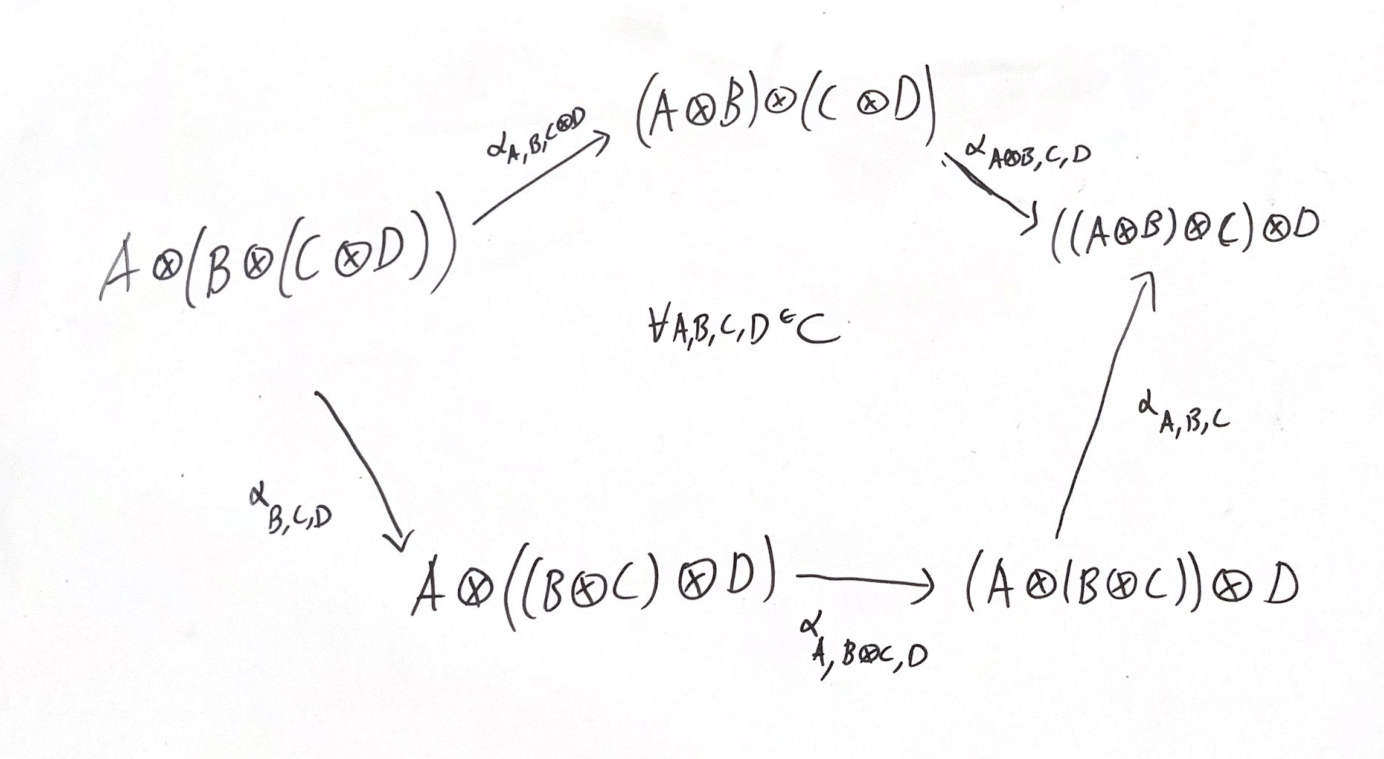
\includegraphics[width=0.7\textwidth]{pent diag.png}
	\caption{Commutative Pentagon Diagram for Monoidal Categories}
\end{figure}


In the context of any nontrivial anyonic system, we intrepret the bifunctor applied to two objects (or tensor product) as being a fusion of two anyons. The identity object represents a trivial fusion. That is, when fusing any particle with the identity, it is equivalent to think that no fusion is happening at all, since the statistic of the fused anyon will not change with respect to the non-identity anyon. The natural isomorphisms reflect physical assertions we make about fusions between the identity and non-identity anyon types. While it is tempting to think that the objects in the category represent the anyons themselves, they actually represent distinct anyon types. More specifically, an anyon's type is distinguished by its statistics. So, viewing anyonic systems through this lens allows us to make conclusions about all anyons who obeys statistics perscribed by their objects. For more information on the explict link between monoidal category theory and boarder physical systems, see \cite{Rose3}

In order to aptly set up our discussion of Fibonacci anyons, we need to further specify our monoidial category. First, we let the objects of this category be the set $\{e,\tau\}$. Then we explicitly define our bifunctor to have the following form:

\begin{equation}
	\begin{aligned}
		\tau \otimes \tau = 1\oplus \tau
	\end{aligned}
\end{equation}

Anyons of type $\tau$ are specifically referred to as the Fibonacci anyons. Our interpretation for the above equation is inherently physical. When Fibonacci anyons fuse together, the resulting quasiparticle does not necessarily obey the same statistics. In our category, there are only two types of anyons, meaning that the fusion of two $\tau$ anyons will yield an anyon of type $e$ or type $\tau$. The direct sum is a probabilistic quantum superposition of states, where each state is represented by the statistics that anyons obey. In this sense, there is some likelihood that the fusion of two Fibonacci anyons will yield another Fibonacci anyon or the fusion will degrade into the vacuum state (we say in this case that the Fibonacci anyons are their own antiparticles). We refer to each outcome as a multi-fushion channel.

In general, we have multiple anyons to keep track of, and the fusion rules ascribed to the system play out in successive fusions of neighboring quasiparticles. If we have $n$ Fibonacci anyons and we track their statistics through their fusion channels, it is no surprise that for any resulting anyon type, the process of arriving to it was not unique. We represent each possible scenario with a diagram, known as a fushion path.

\begin{example}\end{example} 
Suppose we have three Fibonacci anyons. We can illustrate the following fusion paths to see every possible way we can fuse these anyons.

\begin{figure}[H]
	\centering
	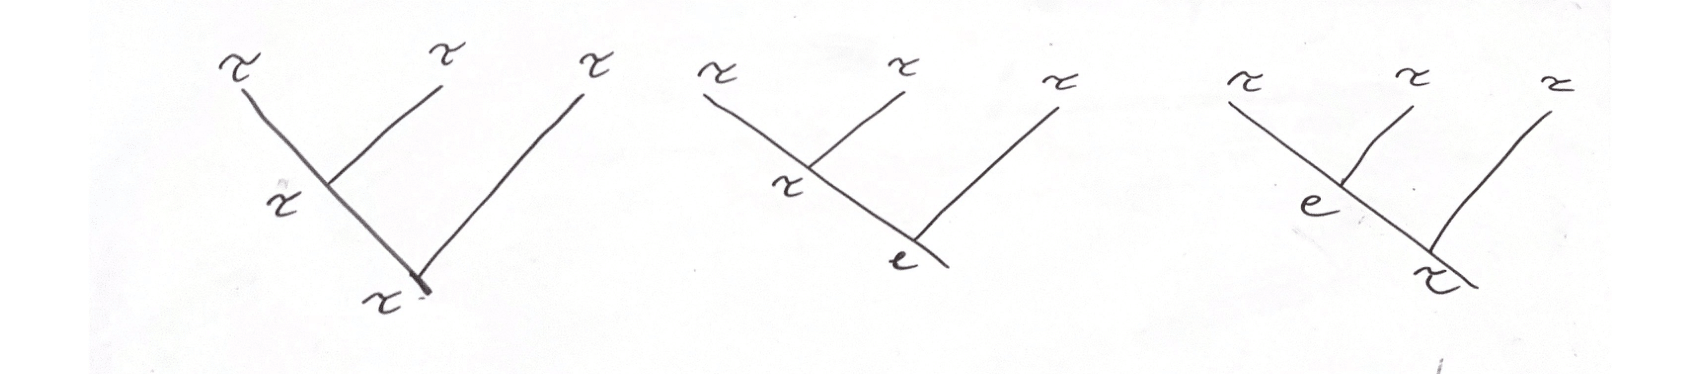
\includegraphics[width=0.7\textwidth]{treebasis.png}
	\caption{These tree diagrams are labelled according to the fusions rules of Fibonacci anyons.}
\end{figure}


These diagrams represent different states of the same anyonic system. If the resulting anyon type is $\tau$, we refer to the fusion tree as representing a ground state. We can use the fusion trees to characterize all possible ground states (degeneracy), and therefore, these trees represent an orthonormal basis of the ground-state manifold\cite{Trebst}. We refer to this as the fusion tree basis of the anyonic system. We can then utilize a combinatorial technique to count the number of ground states (given a fixed number of anyons). If we have $n$ anyons, and $F_n$ represents the number of ground states, we can see that last fusion must have been one of two possible fusions: $\tau\otimes \tau$ or $e \otimes \tau$. In the former scenario, the number of ways for this to happen is characterized by $F_{n-1}$ and in the latter scenario, the number of ways for this to happen is $F_{n-2}$. In general, we can see that the degeneracy of the ground states is exactly equal to the $n^{th}$ Fibonacci number.

Thus far, we have implictly considered fusions to occur successively as outlined by our fusion tree basis. However, in a physical scenario, there is nothing stopping anyons from fusing in a different order. We can use our pentagon diagram above to guide our intuition into how we swap between fusion trees.

Since both fusion trees represent orthonormal bases of the same ground state, they msut be related by a unitary transformation. We call such a transformation an $F$-move. $F$-moves take on the form of matrices whose entries can be specified by a system of equations that generalizes for any $n$ anyon systems. These equations are referred to as the pentagons and they are desugned to explicitly make use of the commutative diagram of the category we are working in. It is worth noting that for each application of an $F$-move, we only alter a component of the fushion tree, not the entire tree. Specifically, we view $F$ matrices as being defined on four anyons: three anyons that will be fused in the tree and one that will be the final result. The $F$ matrix denoted $F^{abc}_d$ defines an $F$ move that exchanges the order of fusion from $(a\otimes b)\otimes c$ to $a\otimes(b\otimes c)$ as depected below.

\begin{figure}[H]
	\centering
	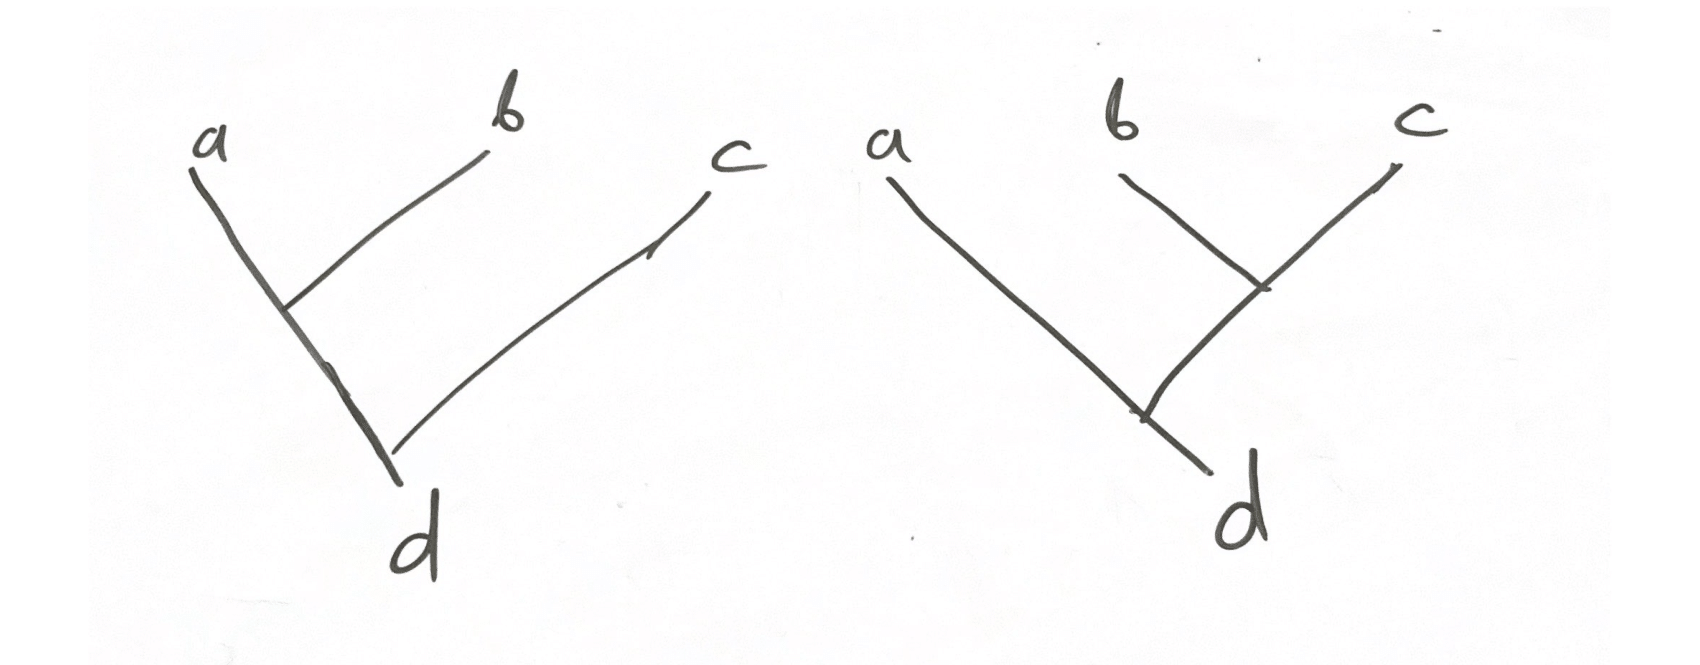
\includegraphics[width=0.7\textwidth]{differentftb}
	\caption{Both tree diagrams represent a different fusion order on the same anyon types.}
\end{figure}

In this sense, we can intuitivley decompose each tree basis into components affected by $F$-moves and components that are not. If we think of each fushion tree as being comprised of two sub-trees joined by one edge, this decomposition is straight forward: For each type of anyon ($e$ and $\tau$), the fusion tree basis for each subtrees (on fewer quasiparticles) can be discerned and then written as a tensor product (corresponding to the whole tree). We take the direct sum of both tensors (one for $e$ and one for $\tau$) to reflect all possible scenarios.

In general, solving for the pentagons is actually quite difficult. But through the study of Fibonacci anyons, we can make some simplifications to our set up. If any anyon is the identity type, our resulting matrix must be the identity matrix (since fusion with this does not impact the overall system). To this end, we need only solve for the transformation matrix when all particles involved are of type $\tau$. The general pentagon equation is written

\begin{equation}
	\begin{aligned}
		[F^{\tau\tau c}_\tau]_{da}[F^{a\tau\tau}_\tau]_{cb} = [F^{\tau\tau \tau}_d]_{cf}[F^{\tau f\tau}_\tau]_{db}[F^{\tau\tau\tau}_b]_{fa}\cite{Trebst}
	\end{aligned}
\end{equation}
where $a,b,c,d,f\in\{e,\tau\}$. Note that the matrices indices are tracked by noninteger values, however the meaning of the subscript is identifies $e$ with the first row/column and $\tau$ with the second row/column. Using the simplfications discussed in the previous paragraph, we can set $b=c=e$ and $a=d=f=\tau$ in order to reduce our equation to 

\begin{equation}
	\begin{aligned}
		[F^{\tau\tau\tau}_\tau]_{11} = [F^{\tau\tau\tau}_\tau]_{12}[F^{\tau\tau\tau}_\tau]_{21}
	\end{aligned}
\end{equation}

where we switch the matrix indices for their integer values for ease of interpretation. Since this transformation is unitary (and based on the number of anyon types, $2\times 2$), we conclude that this matrix must have the following form:

\begin{equation}
	\begin{aligned}
		F^{\tau\tau\tau}_\tau = \begin{bmatrix}
									\frac{1}{\Phi} & \frac{1}{\sqrt{\Phi}}\\
									\frac{1}{\sqrt{\Phi}} & -\frac{1}{\Phi}
								\end{bmatrix}
	\end{aligned}
\end{equation}

where $\Phi$ is the golden ratio.

Now that we have established ways to characterize fusions of anyons, we can intermix discussion of braidings. If we consider a particle exchange of two anyons in an anyonic system, we can expect that the ground state resulting from the fusion of all anyons in the system may be impacted. As such, we can view these transformations in the same context as our $F$-matrices. When two anyons braid, we have a unitary transformation acting on our orthonormal basis of our ground states. Therefore, we can view this transformation in the context of matrix multiplication, and we refer to these anyon braiding matrices as $R$-matrices. We will show that we can obtain a representation of the braid group through combining $F$-matrices and $R$-matrices in a meaningful way. When we incorporate braiding into our problem, we can rigorously define the operation in the concept of a new category.


\begin{definition}
	A \textbf{braided monoidal category} is a monoidal category equipped with a "braiding," $\beta$, which is an isomorphism that satisfies the following commutative diagram:
\end{definition}

\begin{figure}[H]
	\centering
	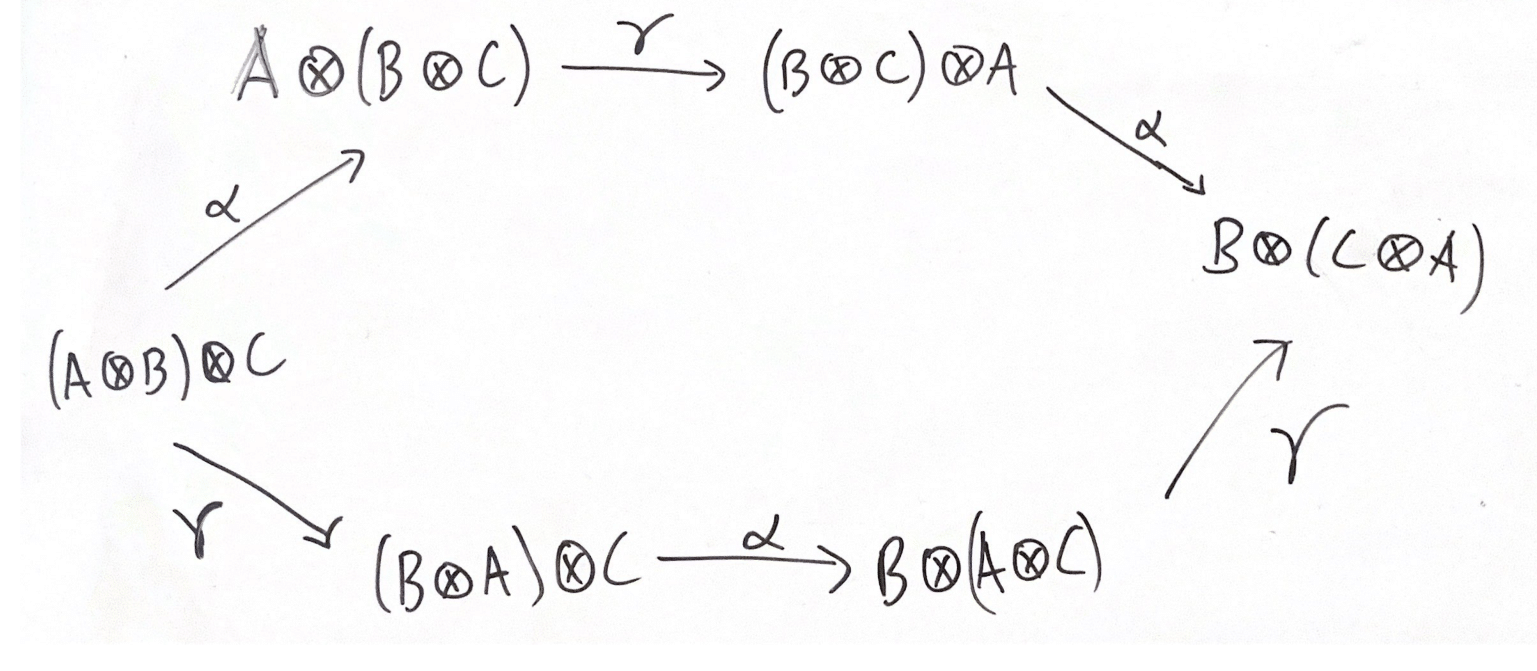
\includegraphics[width=0.7\textwidth]{hexdiag}
	\caption{Hexagonal Commutative Diagram for Braiding Monoidal Categories}
\end{figure}

where $\alpha$ is the associator of the category. For more details on the general properties, see \cite{Joyal}. One idea worth emphasizing here is that in these categories, braiding and fusion are compatible with one another. The best way to think about this is much like the Reidmeister rules from earlier. We can treat tree diagrams as embeddings in three dimensional space, an manipulate the diagram in ways that preserve their structure (isotopy). We can pull fusions under or over braids in the following way:

\begin{figure}[H]
	\centering
	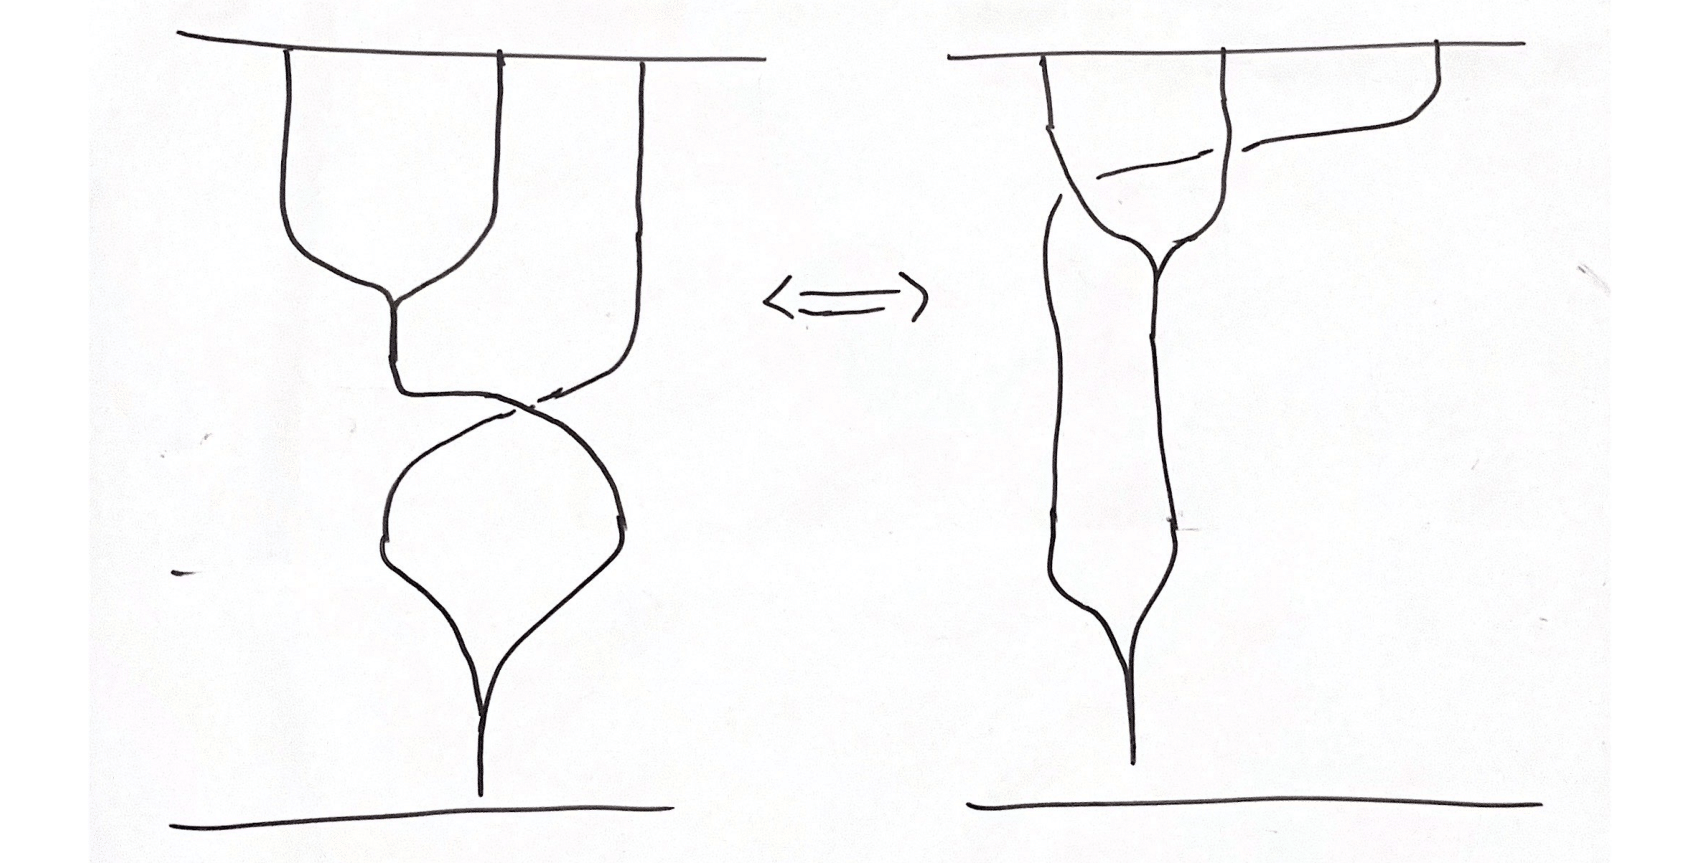
\includegraphics[width=0.7\textwidth]{fusethrubraid.png}
	\caption{Compatibility of braiding and fusion.}
\end{figure}

%As we have seen in our prior discussion of representations of braids defined on the space of wave functions, we can view the action of $R$-matrices not just on our fusion tree basis but the concrete vector space of ground states. That is, since $R$-moves change tree bases, the $R$-matrices must transform orthonormal basis vectors corresponding to them in an identical way. In general, these spaces have a larger dimension than one, and we have nontrivial linear combinations. 

These $R$-matrices can be solved for by utilizing the relations specified in the commutative diagram of the category. If we label $R^{a,b}_c$ as the $R$-matrix who braids the anyons labeled by $a$ and $b$ with total charge $c$, then the following system of equations are referred to as the hexagons:

\begin{equation}
	\begin{aligned}
		R^{\tau,\tau}_c [F^{\tau\tau\tau}_\tau]_{ca}R^{\tau,\tau}_a = \sum_b [F^{\tau\tau\tau}_\tau]_{cb}R^{\tau,b}_\tau[F^{\tau\tau\tau}_\tau]_{ba} \cite{Trebst}
	\end{aligned}
\end{equation}

where $a,b,c\in\{e,\tau\}$ and we again reference the matrix entries based on the row/column values perscribed to $e$ and $\tau$ above. We also note that braiding any $e$ anyon around a $\tau$ anyon leads to no change, and should mean the $R$-matrices would be the identity matrix. Therefore, we get a complicated system of equations.

\begin{equation}
	\begin{aligned}
		(R^{\tau,\tau}_e)^2\frac{1}{\Phi} = R^{\tau,\tau}_\tau\frac{1}{\Phi} + \frac{1}{\Phi^2}
	\end{aligned}
\end{equation}
\begin{equation}
	\begin{aligned}
		R^{\tau,\tau}_eR^{\tau,\tau}_\tau\frac{1}{\sqrt{\Phi}} = (1-R^{\tau,\tau}_\tau)\frac{1}{\Phi^\frac{3}{2}} 
	\end{aligned}
\end{equation}
\begin{equation}
	\begin{aligned}
		-(R^{\tau,\tau}_e)^2\frac{1}{\Phi} = R^{\tau,\tau}_\tau\frac{1}{\Phi^2}+\frac{1}{\Phi}
	\end{aligned}
\end{equation}

If we take our state space to be one dimensional, the $R$-matrices are complex numbers, and we can characterize them much more easily with the solutions $R^{\tau\tau}_e = e^{i\frac{4\pi}{5}}$ and $R^{\tau\tau}_\tau = e^{i\frac{-3\pi}{5}}$. The general braid representation matrices take the form of 

\begin{equation}
	\begin{aligned}
		B = F^{-1}R F
	\end{aligned}
\end{equation}

where we interpret our $F$ matrices as change of basis transformation on the underlying state space and $R$ represents an exchange of two anyons. A more geometrical interpretation for this action is to take two anyons, denoted by the type $\tau$, to fuse them together, then interchange them, and then to unfuse them (preserving the interchange). 

\begin{figure}[H]
	\centering
	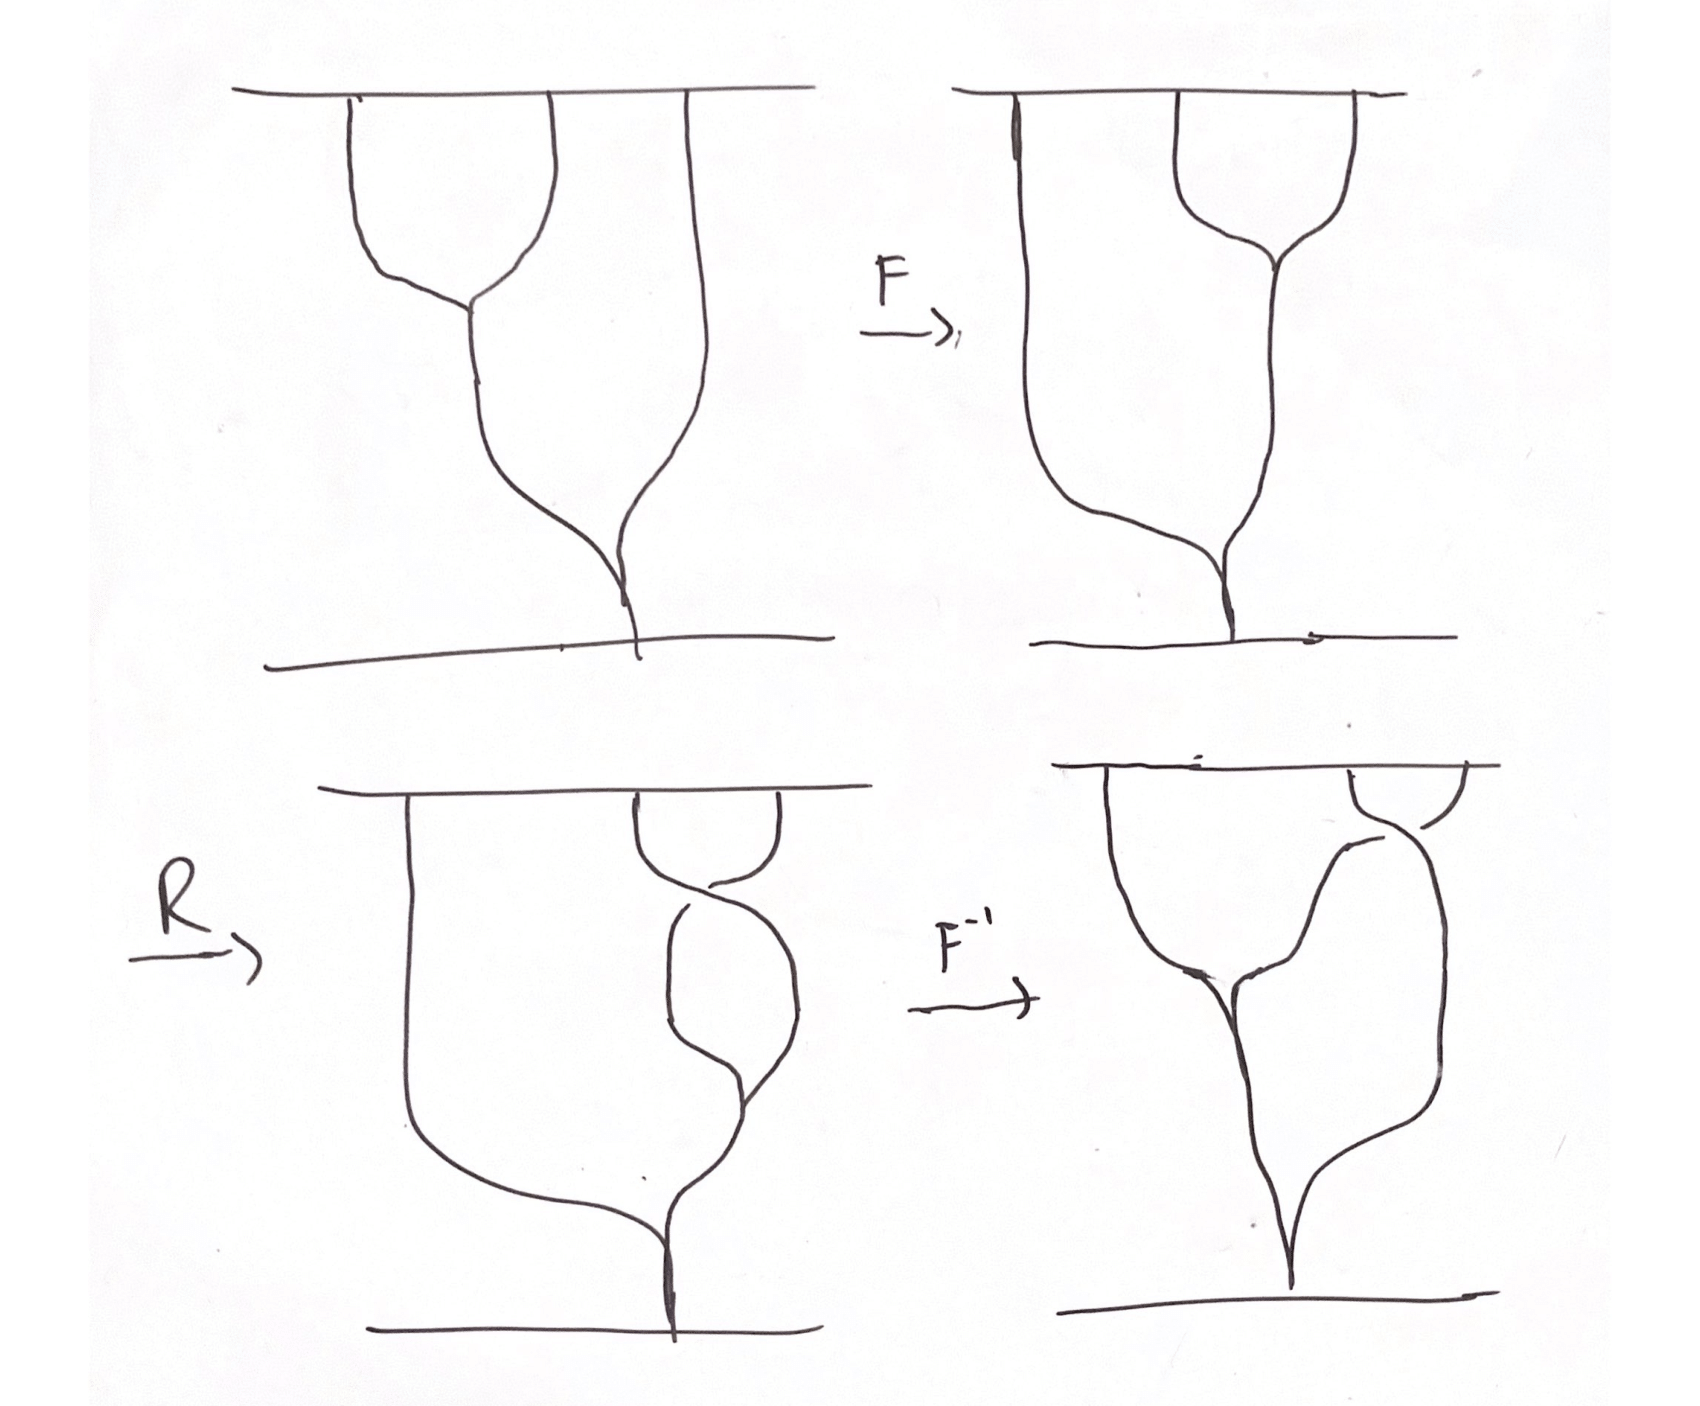
\includegraphics[width=0.7\textwidth]{braid.png}
	\caption{The process of braiding decomposed into fusion and anyon exchanges.}
\end{figure}

At this point, it should be noted that without more specificity it is quite difficult to explicitly compute these matrices. We will use a simple example to illustrate what the general approach would be.

\begin{example}
\end{example}
Suppose that we have two adjacent $\tau$ anyons whose collective charge is $\tau$ after being fused. We label the intermediately fused anyons as by the markers $a,b,c$ successively, we can identify five valid choices: $\{e\tau e,\tau\tau e, e\tau\tau, \tau e\tau, \tau\tau\tau\}$. These states will form the basis of our vector space.

\begin{figure}[H]
	\centering
	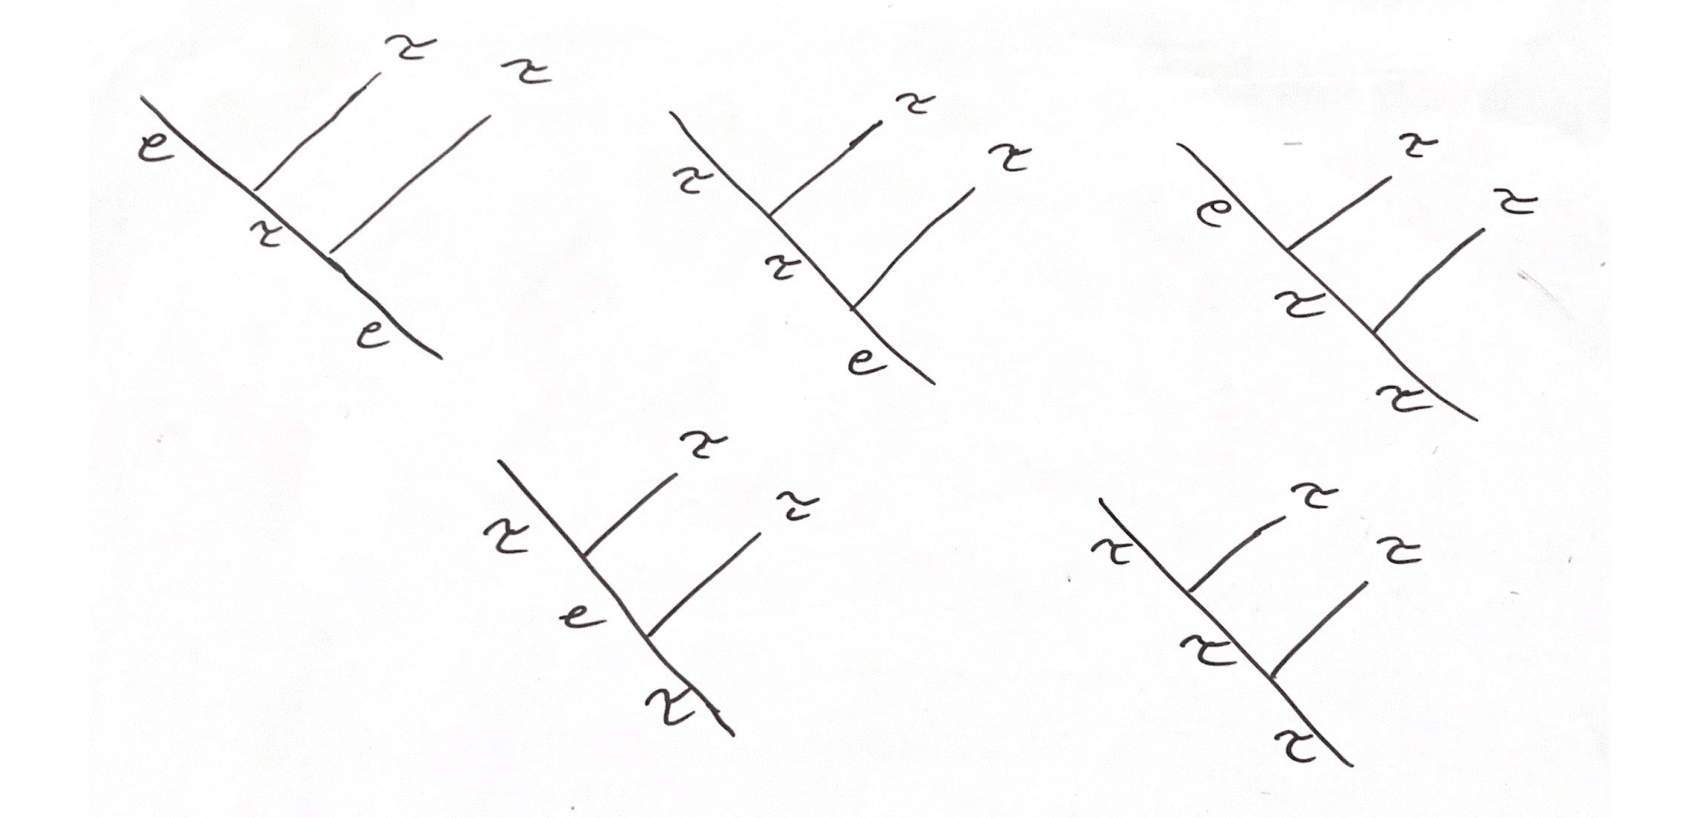
\includegraphics[width=0.7\textwidth]{fivetrees.png}
	\caption{These five trees represent all valid choices for labeling intermediate fusions.}
\end{figure}

If we use the $F$-move that fuses our anyons together, we end up with a new choice of the intermediate fusions: $\{e\tau e,\tau\tau e, e\tau\tau, \tau e\tau, \tau\tau\tau\}$. This transformation is represented by the following $F$-matrix:

\begin{equation}
	\begin{aligned}
		F = \begin{bmatrix}
				1 & 0 & 0 & 0 & 0 \\
				0 & 1 & 0 & 0 & 0 \\
				0 & 0 & 1 & 0 & 0 \\
				0 & 0 & 0 & \frac{1}{\Phi} & \frac{1}{\sqrt{\Phi}}\\
				0 & 0 & 0 &\frac{1}{\sqrt{\Phi}} & -\frac{1}{\Phi}
			\end{bmatrix}\cite{Trebst}
	\end{aligned}
\end{equation}

with respect to the basis of states described. By identifying the $R$-move necessary to exchange the anyons given its state, we see that our $R$-matrix takes the following form:

\begin{equation}
	\begin{aligned}
		R = \begin{bmatrix}
				e^{i\frac{4\pi}{5}} & 0 & 0 & 0 & 0 \\
				0 & e^{i\frac{-3\pi}{5}} & 0 & 0 & 0 \\
				0 & 0 & e^{i\frac{-3\pi}{5}} & 0 & 0 \\
				0 & 0 & 0 & e^{i\frac{4\pi}{5}} & 0\\
				0 & 0 & 0 & 0 &e^{i\frac{-3\pi}{5}} 
			\end{bmatrix}
	\end{aligned}
\end{equation}

Therefore, we can construct the braid matrix

\begin{equation}
	\begin{aligned}
		B = \begin{bmatrix}
				e^{i\frac{4\pi}{5}} & 0 & 0 & 0 & 0 \\
				0 & e^{i\frac{-3\pi}{5}} & 0 & 0 & 0 \\
				0 & 0 & e^{i\frac{-3\pi}{5}} & 0 & 0 \\
				0 & 0 & 0 & \frac{-e^{i\frac{4\pi}{5}}}{\Phi^2} + \frac{-e^{i\frac{-3\pi}{5}}}{\Phi}& \frac{-e^{i\frac{4\pi}{5}}}{\Phi^\frac{3}{2}} + \frac{e^{i\frac{-3\pi}{5}}}{\Phi^\frac{3}{2}}\\
				0 & 0 & 0&\frac{-e^{i\frac{4\pi}{5}}}{\Phi^\frac{3}{2}} + \frac{e^{i\frac{-3\pi}{5}}}{\Phi^\frac{3}{2}} &\frac{-e^{i\frac{4\pi}{5}}}{\Phi^2} + \frac{-e^{i\frac{-3\pi}{5}}}{\Phi}
			\end{bmatrix}
	\end{aligned}
\end{equation}

This matrix characterizes the behavior of two Fibonacci anyons braiding with one another given the ground states of our two anyons are all one dimensional. If we were to look at all the anyons in our system, we would see more complicated matrices take form. Most easily, we could generalize these interactions to more anyons in the system if we were to consider more fusions and exchanges happening successively. Such a braid matrix would take the following form

\begin{equation}
	\begin{aligned}
		B = \prod_i F_i^{-1}R_iF_i
	\end{aligned}
\end{equation}

where each factor in the product represents a single exchange of two specified anyons specified by the choice of $F_i$ and $R_i$. It is not unreasonable to see that given more specification on our space we could construct a representation using matrices of these form.